% Options for packages loaded elsewhere
\PassOptionsToPackage{unicode}{hyperref}
\PassOptionsToPackage{hyphens}{url}
\PassOptionsToPackage{dvipsnames,svgnames,x11names}{xcolor}
%
\documentclass[
  11pt,
  a4paper,
  DIV=11,
  numbers=noendperiod]{scrartcl}

\usepackage{amsmath,amssymb}
\usepackage{iftex}
\ifPDFTeX
  \usepackage[T1]{fontenc}
  \usepackage[utf8]{inputenc}
  \usepackage{textcomp} % provide euro and other symbols
\else % if luatex or xetex
  \usepackage{unicode-math}
  \defaultfontfeatures{Scale=MatchLowercase}
  \defaultfontfeatures[\rmfamily]{Ligatures=TeX,Scale=1}
\fi
\usepackage{lmodern}
\ifPDFTeX\else  
    % xetex/luatex font selection
\fi
% Use upquote if available, for straight quotes in verbatim environments
\IfFileExists{upquote.sty}{\usepackage{upquote}}{}
\IfFileExists{microtype.sty}{% use microtype if available
  \usepackage[]{microtype}
  \UseMicrotypeSet[protrusion]{basicmath} % disable protrusion for tt fonts
}{}
\makeatletter
\@ifundefined{KOMAClassName}{% if non-KOMA class
  \IfFileExists{parskip.sty}{%
    \usepackage{parskip}
  }{% else
    \setlength{\parindent}{0pt}
    \setlength{\parskip}{6pt plus 2pt minus 1pt}}
}{% if KOMA class
  \KOMAoptions{parskip=half}}
\makeatother
\usepackage{xcolor}
\usepackage[lmargin=2cm,rmargin=2cm,tmargin=2cm,bmargin=2cm]{geometry}
\setlength{\emergencystretch}{3em} % prevent overfull lines
\setcounter{secnumdepth}{-\maxdimen} % remove section numbering
% Make \paragraph and \subparagraph free-standing
\ifx\paragraph\undefined\else
  \let\oldparagraph\paragraph
  \renewcommand{\paragraph}[1]{\oldparagraph{#1}\mbox{}}
\fi
\ifx\subparagraph\undefined\else
  \let\oldsubparagraph\subparagraph
  \renewcommand{\subparagraph}[1]{\oldsubparagraph{#1}\mbox{}}
\fi

\usepackage{color}
\usepackage{fancyvrb}
\newcommand{\VerbBar}{|}
\newcommand{\VERB}{\Verb[commandchars=\\\{\}]}
\DefineVerbatimEnvironment{Highlighting}{Verbatim}{commandchars=\\\{\}}
% Add ',fontsize=\small' for more characters per line
\usepackage{framed}
\definecolor{shadecolor}{RGB}{241,243,245}
\newenvironment{Shaded}{\begin{snugshade}}{\end{snugshade}}
\newcommand{\AlertTok}[1]{\textcolor[rgb]{0.68,0.00,0.00}{#1}}
\newcommand{\AnnotationTok}[1]{\textcolor[rgb]{0.37,0.37,0.37}{#1}}
\newcommand{\AttributeTok}[1]{\textcolor[rgb]{0.40,0.45,0.13}{#1}}
\newcommand{\BaseNTok}[1]{\textcolor[rgb]{0.68,0.00,0.00}{#1}}
\newcommand{\BuiltInTok}[1]{\textcolor[rgb]{0.00,0.23,0.31}{#1}}
\newcommand{\CharTok}[1]{\textcolor[rgb]{0.13,0.47,0.30}{#1}}
\newcommand{\CommentTok}[1]{\textcolor[rgb]{0.37,0.37,0.37}{#1}}
\newcommand{\CommentVarTok}[1]{\textcolor[rgb]{0.37,0.37,0.37}{\textit{#1}}}
\newcommand{\ConstantTok}[1]{\textcolor[rgb]{0.56,0.35,0.01}{#1}}
\newcommand{\ControlFlowTok}[1]{\textcolor[rgb]{0.00,0.23,0.31}{#1}}
\newcommand{\DataTypeTok}[1]{\textcolor[rgb]{0.68,0.00,0.00}{#1}}
\newcommand{\DecValTok}[1]{\textcolor[rgb]{0.68,0.00,0.00}{#1}}
\newcommand{\DocumentationTok}[1]{\textcolor[rgb]{0.37,0.37,0.37}{\textit{#1}}}
\newcommand{\ErrorTok}[1]{\textcolor[rgb]{0.68,0.00,0.00}{#1}}
\newcommand{\ExtensionTok}[1]{\textcolor[rgb]{0.00,0.23,0.31}{#1}}
\newcommand{\FloatTok}[1]{\textcolor[rgb]{0.68,0.00,0.00}{#1}}
\newcommand{\FunctionTok}[1]{\textcolor[rgb]{0.28,0.35,0.67}{#1}}
\newcommand{\ImportTok}[1]{\textcolor[rgb]{0.00,0.46,0.62}{#1}}
\newcommand{\InformationTok}[1]{\textcolor[rgb]{0.37,0.37,0.37}{#1}}
\newcommand{\KeywordTok}[1]{\textcolor[rgb]{0.00,0.23,0.31}{#1}}
\newcommand{\NormalTok}[1]{\textcolor[rgb]{0.00,0.23,0.31}{#1}}
\newcommand{\OperatorTok}[1]{\textcolor[rgb]{0.37,0.37,0.37}{#1}}
\newcommand{\OtherTok}[1]{\textcolor[rgb]{0.00,0.23,0.31}{#1}}
\newcommand{\PreprocessorTok}[1]{\textcolor[rgb]{0.68,0.00,0.00}{#1}}
\newcommand{\RegionMarkerTok}[1]{\textcolor[rgb]{0.00,0.23,0.31}{#1}}
\newcommand{\SpecialCharTok}[1]{\textcolor[rgb]{0.37,0.37,0.37}{#1}}
\newcommand{\SpecialStringTok}[1]{\textcolor[rgb]{0.13,0.47,0.30}{#1}}
\newcommand{\StringTok}[1]{\textcolor[rgb]{0.13,0.47,0.30}{#1}}
\newcommand{\VariableTok}[1]{\textcolor[rgb]{0.07,0.07,0.07}{#1}}
\newcommand{\VerbatimStringTok}[1]{\textcolor[rgb]{0.13,0.47,0.30}{#1}}
\newcommand{\WarningTok}[1]{\textcolor[rgb]{0.37,0.37,0.37}{\textit{#1}}}

\providecommand{\tightlist}{%
  \setlength{\itemsep}{0pt}\setlength{\parskip}{0pt}}\usepackage{longtable,booktabs,array}
\usepackage{calc} % for calculating minipage widths
% Correct order of tables after \paragraph or \subparagraph
\usepackage{etoolbox}
\makeatletter
\patchcmd\longtable{\par}{\if@noskipsec\mbox{}\fi\par}{}{}
\makeatother
% Allow footnotes in longtable head/foot
\IfFileExists{footnotehyper.sty}{\usepackage{footnotehyper}}{\usepackage{footnote}}
\makesavenoteenv{longtable}
\usepackage{graphicx}
\makeatletter
\def\maxwidth{\ifdim\Gin@nat@width>\linewidth\linewidth\else\Gin@nat@width\fi}
\def\maxheight{\ifdim\Gin@nat@height>\textheight\textheight\else\Gin@nat@height\fi}
\makeatother
% Scale images if necessary, so that they will not overflow the page
% margins by default, and it is still possible to overwrite the defaults
% using explicit options in \includegraphics[width, height, ...]{}
\setkeys{Gin}{width=\maxwidth,height=\maxheight,keepaspectratio}
% Set default figure placement to htbp
\makeatletter
\def\fps@figure{htbp}
\makeatother

\KOMAoption{captions}{tableheading}
\makeatletter
\makeatother
\makeatletter
\makeatother
\makeatletter
\@ifpackageloaded{caption}{}{\usepackage{caption}}
\AtBeginDocument{%
\ifdefined\contentsname
  \renewcommand*\contentsname{Table of contents}
\else
  \newcommand\contentsname{Table of contents}
\fi
\ifdefined\listfigurename
  \renewcommand*\listfigurename{List of Figures}
\else
  \newcommand\listfigurename{List of Figures}
\fi
\ifdefined\listtablename
  \renewcommand*\listtablename{List of Tables}
\else
  \newcommand\listtablename{List of Tables}
\fi
\ifdefined\figurename
  \renewcommand*\figurename{Figure}
\else
  \newcommand\figurename{Figure}
\fi
\ifdefined\tablename
  \renewcommand*\tablename{Table}
\else
  \newcommand\tablename{Table}
\fi
}
\@ifpackageloaded{float}{}{\usepackage{float}}
\floatstyle{ruled}
\@ifundefined{c@chapter}{\newfloat{codelisting}{h}{lop}}{\newfloat{codelisting}{h}{lop}[chapter]}
\floatname{codelisting}{Listing}
\newcommand*\listoflistings{\listof{codelisting}{List of Listings}}
\makeatother
\makeatletter
\@ifpackageloaded{caption}{}{\usepackage{caption}}
\@ifpackageloaded{subcaption}{}{\usepackage{subcaption}}
\makeatother
\makeatletter
\@ifpackageloaded{tcolorbox}{}{\usepackage[skins,breakable]{tcolorbox}}
\makeatother
\makeatletter
\@ifundefined{shadecolor}{\definecolor{shadecolor}{rgb}{.97, .97, .97}}
\makeatother
\makeatletter
\makeatother
\makeatletter
\makeatother
\ifLuaTeX
  \usepackage{selnolig}  % disable illegal ligatures
\fi
\IfFileExists{bookmark.sty}{\usepackage{bookmark}}{\usepackage{hyperref}}
\IfFileExists{xurl.sty}{\usepackage{xurl}}{} % add URL line breaks if available
\urlstyle{same} % disable monospaced font for URLs
\hypersetup{
  pdftitle={ANALYSIS},
  colorlinks=true,
  linkcolor={blue},
  filecolor={Maroon},
  citecolor={Blue},
  urlcolor={Blue},
  pdfcreator={LaTeX via pandoc}}

\title{ANALYSIS}
\author{}
\date{}

\begin{document}
\maketitle
\ifdefined\Shaded\renewenvironment{Shaded}{\begin{tcolorbox}[frame hidden, sharp corners, breakable, interior hidden, enhanced, borderline west={3pt}{0pt}{shadecolor}, boxrule=0pt]}{\end{tcolorbox}}\fi

quarto install tinytex tlmgr path add

\hypertarget{key-takeaways}{%
\section{KEY TAKEAWAYS}\label{key-takeaways}}

The aim of this project is to analyze internal migration data in Turkey
and investigate the factors such as migration reasons, age, education,
and other variables that influence migration. We conducted our research
using the internal migration and population datasets available on the
Turkish Statistical Institute (TÜİK) website. The conclusions drawn from
this project are outlined in the following points:

\begin{enumerate}
\def\labelenumi{\arabic{enumi}.}
\item
  We had assumed that the highest migration due to retirement would be
  to the Central Anatolia Region or the Aegean Region. To validate this
  assumption, we created a migration value and cause graph. When looking
  at this graph, we observed that the highest migration is to the
  Marmara Region. To obtain more accurate results, we created a
  migration rate and cause graph. In this graph, we see that the highest
  migration is to the Black Sea and Aegean regions. So, we realized that
  part of our assumption is correct. Understanding the importance of
  creating a Rate graph, we concluded that we should make decisions
  based on this graph.
\item
  The age range of the people who migrate the most is seen in the graph
  as 20-24. The age group of the people who migrated the second most is
  seen in the graph as 15-19. In the graph of reasons for migration, the
  most common reason for migration was observed to be education. We can
  reconcile this incident with this situation.
\item
  The visual representation of migration numbers across different
  educational backgrounds highlights a compelling inverse relationship
  between education and migration. Doctoral and primary school-educated
  individuals show lower migration rates compared to high school and
  university-educated individuals. Individuals with higher education
  levels tend to migrate less. The scatter plot analysis reveals a lack
  of a straightforward correlation between the average education level
  and fertility rates across regions in the dataset. While some general
  trends emerge---like higher education levels in certain regions
  coinciding with lower fertility rates---outliers such as Central
  Anatolia and the Mediterranean Region defy these patterns.
\end{enumerate}

\hypertarget{data-preprocessing}{%
\section{DATA PREPROCESSING}\label{data-preprocessing}}

\begin{Shaded}
\begin{Highlighting}[]
\CommentTok{\# importing necessary packages}
\FunctionTok{library}\NormalTok{(tidyverse)}
\FunctionTok{library}\NormalTok{(readxl)}
\FunctionTok{library}\NormalTok{(readr)}
\FunctionTok{library}\NormalTok{(gridExtra)}
\FunctionTok{library}\NormalTok{(dplyr)}

\NormalTok{population }\OtherTok{\textless{}{-}} \FunctionTok{read\_excel}\NormalTok{(}\StringTok{"C:}\SpecialCharTok{\textbackslash{}\textbackslash{}}\StringTok{Users}\SpecialCharTok{\textbackslash{}\textbackslash{}}\StringTok{melek}\SpecialCharTok{\textbackslash{}\textbackslash{}}\StringTok{desktop}\SpecialCharTok{\textbackslash{}\textbackslash{}}\StringTok{DataVizards\_FinalDataFrame.xlsx"}\NormalTok{)}
\FunctionTok{names}\NormalTok{(population) }\OtherTok{\textless{}{-}} \FunctionTok{c}\NormalTok{(}\StringTok{\textquotesingle{}IDD\textquotesingle{}}\NormalTok{,}\StringTok{\textquotesingle{}city\textquotesingle{}}\NormalTok{,}\StringTok{\textquotesingle{}regionid\textquotesingle{}}\NormalTok{,}\StringTok{\textquotesingle{}regions\textquotesingle{}}\NormalTok{,}\StringTok{\textquotesingle{}totalpop\textquotesingle{}}\NormalTok{,}\StringTok{\textquotesingle{}male\textquotesingle{}}\NormalTok{,}\StringTok{\textquotesingle{}female\textquotesingle{}}\NormalTok{,}\StringTok{\textquotesingle{}age04\textquotesingle{}}\NormalTok{,}\StringTok{\textquotesingle{}age59\textquotesingle{}}\NormalTok{,}\StringTok{\textquotesingle{}age1014\textquotesingle{}}\NormalTok{,}\StringTok{\textquotesingle{}age1519\textquotesingle{}}\NormalTok{,}\StringTok{\textquotesingle{}age2024\textquotesingle{}}\NormalTok{,}\StringTok{\textquotesingle{}age2529\textquotesingle{}}\NormalTok{,}\StringTok{\textquotesingle{}age3034\textquotesingle{}}\NormalTok{,}\StringTok{\textquotesingle{}age3539\textquotesingle{}}\NormalTok{,}\StringTok{\textquotesingle{}age4044\textquotesingle{}}\NormalTok{,}\StringTok{\textquotesingle{}otherage\textquotesingle{}}\NormalTok{,}\StringTok{\textquotesingle{}unknowns\textquotesingle{}}\NormalTok{,}\StringTok{\textquotesingle{}doctorate\textquotesingle{}}\NormalTok{,}\StringTok{\textquotesingle{}primaryedu\textquotesingle{}}\NormalTok{,}\StringTok{\textquotesingle{}elementaryedu\textquotesingle{}}\NormalTok{,}\StringTok{\textquotesingle{}highschool\textquotesingle{}}\NormalTok{,}\StringTok{\textquotesingle{}literatebutnoschool\textquotesingle{}}\NormalTok{,}\StringTok{\textquotesingle{}notliterate\textquotesingle{}}\NormalTok{,}\StringTok{\textquotesingle{}middleschool\textquotesingle{}}\NormalTok{,}\StringTok{\textquotesingle{}master\textquotesingle{}}\NormalTok{,}\StringTok{\textquotesingle{}university\textquotesingle{}}\NormalTok{,}\StringTok{\textquotesingle{}fertilityrate\textquotesingle{}}\NormalTok{,}\StringTok{\textquotesingle{}electricity\textquotesingle{}}\NormalTok{,}\StringTok{\textquotesingle{}numberofattempts\textquotesingle{}}\NormalTok{,}\StringTok{\textquotesingle{}housingsalesnumbers\textquotesingle{}}\NormalTok{)}

\NormalTok{region26 }\OtherTok{\textless{}{-}} \FunctionTok{read\_excel}\NormalTok{(}\StringTok{"C:}\SpecialCharTok{\textbackslash{}\textbackslash{}}\StringTok{Users}\SpecialCharTok{\textbackslash{}\textbackslash{}}\StringTok{melek}\SpecialCharTok{\textbackslash{}\textbackslash{}}\StringTok{desktop}\SpecialCharTok{\textbackslash{}\textbackslash{}}\StringTok{DataVizards\_FinalDataFrame.xlsx"}\NormalTok{, }\AttributeTok{sheet =} \StringTok{"Bolge26"}\NormalTok{)}
\FunctionTok{names}\NormalTok{(region26) }\OtherTok{\textless{}{-}} \FunctionTok{c}\NormalTok{(}\StringTok{\textquotesingle{}region\textquotesingle{}}\NormalTok{,}\StringTok{\textquotesingle{}region2id\textquotesingle{}}\NormalTok{,}\StringTok{\textquotesingle{}workforce15plus\textquotesingle{}}\NormalTok{,}\StringTok{\textquotesingle{}workforce1564\textquotesingle{}}\NormalTok{,}\StringTok{\textquotesingle{}usableincome\textquotesingle{}}\NormalTok{)}

\NormalTok{migration }\OtherTok{\textless{}{-}} \FunctionTok{read\_excel}\NormalTok{(}\StringTok{"C:}\SpecialCharTok{\textbackslash{}\textbackslash{}}\StringTok{Users}\SpecialCharTok{\textbackslash{}\textbackslash{}}\StringTok{melek}\SpecialCharTok{\textbackslash{}\textbackslash{}}\StringTok{desktop}\SpecialCharTok{\textbackslash{}\textbackslash{}}\StringTok{DataVizards\_FinalDataFrame.xlsx"}\NormalTok{)}
\NormalTok{population }\OtherTok{\textless{}{-}} \FunctionTok{read\_excel}\NormalTok{(}\StringTok{"C:}\SpecialCharTok{\textbackslash{}\textbackslash{}}\StringTok{Users}\SpecialCharTok{\textbackslash{}\textbackslash{}}\StringTok{melek}\SpecialCharTok{\textbackslash{}\textbackslash{}}\StringTok{desktop}\SpecialCharTok{\textbackslash{}\textbackslash{}}\StringTok{DataVizards\_FinalDataFrame.xlsx"}\NormalTok{)}
\FunctionTok{names}\NormalTok{(population) }\OtherTok{\textless{}{-}} \FunctionTok{c}\NormalTok{(}\StringTok{\textquotesingle{}IDD\textquotesingle{}}\NormalTok{,}\StringTok{\textquotesingle{}city\textquotesingle{}}\NormalTok{,}\StringTok{\textquotesingle{}regionid\textquotesingle{}}\NormalTok{,}\StringTok{\textquotesingle{}regions\textquotesingle{}}\NormalTok{,}\StringTok{\textquotesingle{}totalpop\textquotesingle{}}\NormalTok{,}\StringTok{\textquotesingle{}male\textquotesingle{}}\NormalTok{,}\StringTok{\textquotesingle{}female\textquotesingle{}}\NormalTok{,}\StringTok{\textquotesingle{}age04\textquotesingle{}}\NormalTok{,}\StringTok{\textquotesingle{}age59\textquotesingle{}}\NormalTok{,}\StringTok{\textquotesingle{}age1014\textquotesingle{}}\NormalTok{,}\StringTok{\textquotesingle{}age1519\textquotesingle{}}\NormalTok{,}\StringTok{\textquotesingle{}age2024\textquotesingle{}}\NormalTok{,}\StringTok{\textquotesingle{}age2529\textquotesingle{}}\NormalTok{,}\StringTok{\textquotesingle{}age3034\textquotesingle{}}\NormalTok{,}\StringTok{\textquotesingle{}age3539\textquotesingle{}}\NormalTok{,}\StringTok{\textquotesingle{}age4044\textquotesingle{}}\NormalTok{,}\StringTok{\textquotesingle{}otherage\textquotesingle{}}\NormalTok{,}\StringTok{\textquotesingle{}unknowns\textquotesingle{}}\NormalTok{,}\StringTok{\textquotesingle{}doctorate\textquotesingle{}}\NormalTok{,}\StringTok{\textquotesingle{}primaryedu\textquotesingle{}}\NormalTok{,}\StringTok{\textquotesingle{}elementaryedu\textquotesingle{}}\NormalTok{,}\StringTok{\textquotesingle{}highschool\textquotesingle{}}\NormalTok{,}\StringTok{\textquotesingle{}literatebutnoschool\textquotesingle{}}\NormalTok{,}\StringTok{\textquotesingle{}notliterate\textquotesingle{}}\NormalTok{,}\StringTok{\textquotesingle{}middleschool\textquotesingle{}}\NormalTok{,}\StringTok{\textquotesingle{}master\textquotesingle{}}\NormalTok{,}\StringTok{\textquotesingle{}university\textquotesingle{}}\NormalTok{,}\StringTok{\textquotesingle{}fertilityrate\textquotesingle{}}\NormalTok{,}\StringTok{\textquotesingle{}electricity\textquotesingle{}}\NormalTok{,}\StringTok{\textquotesingle{}numberofattempts\textquotesingle{}}\NormalTok{,}\StringTok{\textquotesingle{}housingsalesnumbers\textquotesingle{}}\NormalTok{)}

\NormalTok{region26 }\OtherTok{\textless{}{-}} \FunctionTok{read\_excel}\NormalTok{(}\StringTok{"C:}\SpecialCharTok{\textbackslash{}\textbackslash{}}\StringTok{Users}\SpecialCharTok{\textbackslash{}\textbackslash{}}\StringTok{melek}\SpecialCharTok{\textbackslash{}\textbackslash{}}\StringTok{desktop}\SpecialCharTok{\textbackslash{}\textbackslash{}}\StringTok{DataVizards\_FinalDataFrame.xlsx"}\NormalTok{, }\AttributeTok{sheet =} \StringTok{"Bolge26"}\NormalTok{)}
\FunctionTok{names}\NormalTok{(region26) }\OtherTok{\textless{}{-}} \FunctionTok{c}\NormalTok{(}\StringTok{\textquotesingle{}region\textquotesingle{}}\NormalTok{,}\StringTok{\textquotesingle{}region2id\textquotesingle{}}\NormalTok{,}\StringTok{\textquotesingle{}workforce15plus\textquotesingle{}}\NormalTok{,}\StringTok{\textquotesingle{}workforce1564\textquotesingle{}}\NormalTok{,}\StringTok{\textquotesingle{}usableincome\textquotesingle{}}\NormalTok{)}

\NormalTok{migration }\OtherTok{\textless{}{-}} \FunctionTok{read\_excel}\NormalTok{(}\StringTok{"C:}\SpecialCharTok{\textbackslash{}\textbackslash{}}\StringTok{Users}\SpecialCharTok{\textbackslash{}\textbackslash{}}\StringTok{melek}\SpecialCharTok{\textbackslash{}\textbackslash{}}\StringTok{desktop}\SpecialCharTok{\textbackslash{}\textbackslash{}}\StringTok{DataVizards\_FinalDataFrame.xlsx"}\NormalTok{, }\AttributeTok{sheet =} \StringTok{"Goc Bilgileri"}\NormalTok{)}

\NormalTok{population }\OtherTok{\textless{}{-}} \FunctionTok{read\_excel}\NormalTok{(}\StringTok{"C:}\SpecialCharTok{\textbackslash{}\textbackslash{}}\StringTok{Users}\SpecialCharTok{\textbackslash{}\textbackslash{}}\StringTok{melek}\SpecialCharTok{\textbackslash{}\textbackslash{}}\StringTok{desktop}\SpecialCharTok{\textbackslash{}\textbackslash{}}\StringTok{DataVizards\_FinalDataFrame.xlsx"}\NormalTok{)}
\FunctionTok{names}\NormalTok{(population) }\OtherTok{\textless{}{-}} \FunctionTok{c}\NormalTok{(}\StringTok{\textquotesingle{}IDD\textquotesingle{}}\NormalTok{,}\StringTok{\textquotesingle{}city\textquotesingle{}}\NormalTok{,}\StringTok{\textquotesingle{}regionid\textquotesingle{}}\NormalTok{,}\StringTok{\textquotesingle{}regions\textquotesingle{}}\NormalTok{,}\StringTok{\textquotesingle{}totalpop\textquotesingle{}}\NormalTok{,}\StringTok{\textquotesingle{}male\textquotesingle{}}\NormalTok{,}\StringTok{\textquotesingle{}female\textquotesingle{}}\NormalTok{,}\StringTok{\textquotesingle{}age04\textquotesingle{}}\NormalTok{,}\StringTok{\textquotesingle{}age59\textquotesingle{}}\NormalTok{,}\StringTok{\textquotesingle{}age1014\textquotesingle{}}\NormalTok{,}\StringTok{\textquotesingle{}age1519\textquotesingle{}}\NormalTok{,}\StringTok{\textquotesingle{}age2024\textquotesingle{}}\NormalTok{,}\StringTok{\textquotesingle{}age2529\textquotesingle{}}\NormalTok{,}\StringTok{\textquotesingle{}age3034\textquotesingle{}}\NormalTok{,}\StringTok{\textquotesingle{}age3539\textquotesingle{}}\NormalTok{,}\StringTok{\textquotesingle{}age4044\textquotesingle{}}\NormalTok{,}\StringTok{\textquotesingle{}otherage\textquotesingle{}}\NormalTok{,}\StringTok{\textquotesingle{}unknowns\textquotesingle{}}\NormalTok{,}\StringTok{\textquotesingle{}doctorate\textquotesingle{}}\NormalTok{,}\StringTok{\textquotesingle{}primaryedu\textquotesingle{}}\NormalTok{,}\StringTok{\textquotesingle{}elementaryedu\textquotesingle{}}\NormalTok{,}\StringTok{\textquotesingle{}highschool\textquotesingle{}}\NormalTok{,}\StringTok{\textquotesingle{}literatebutnoschool\textquotesingle{}}\NormalTok{,}\StringTok{\textquotesingle{}notliterate\textquotesingle{}}\NormalTok{,}\StringTok{\textquotesingle{}middleschool\textquotesingle{}}\NormalTok{,}\StringTok{\textquotesingle{}master\textquotesingle{}}\NormalTok{,}\StringTok{\textquotesingle{}university\textquotesingle{}}\NormalTok{,}\StringTok{\textquotesingle{}fertilityrate\textquotesingle{}}\NormalTok{,}\StringTok{\textquotesingle{}electricity\textquotesingle{}}\NormalTok{,}\StringTok{\textquotesingle{}numberofattempts\textquotesingle{}}\NormalTok{,}\StringTok{\textquotesingle{}housingsalesnumbers\textquotesingle{}}\NormalTok{)}

\NormalTok{region26 }\OtherTok{\textless{}{-}} \FunctionTok{read\_excel}\NormalTok{(}\StringTok{"C:}\SpecialCharTok{\textbackslash{}\textbackslash{}}\StringTok{Users}\SpecialCharTok{\textbackslash{}\textbackslash{}}\StringTok{melek}\SpecialCharTok{\textbackslash{}\textbackslash{}}\StringTok{desktop}\SpecialCharTok{\textbackslash{}\textbackslash{}}\StringTok{DataVizards\_FinalDataFrame.xlsx"}\NormalTok{, }\AttributeTok{sheet =} \StringTok{"Bolge26"}\NormalTok{)}
\FunctionTok{names}\NormalTok{(region26) }\OtherTok{\textless{}{-}} \FunctionTok{c}\NormalTok{(}\StringTok{\textquotesingle{}region\textquotesingle{}}\NormalTok{,}\StringTok{\textquotesingle{}region2id\textquotesingle{}}\NormalTok{,}\StringTok{\textquotesingle{}workforce15plus\textquotesingle{}}\NormalTok{,}\StringTok{\textquotesingle{}workforce1564\textquotesingle{}}\NormalTok{,}\StringTok{\textquotesingle{}usableincome\textquotesingle{}}\NormalTok{)}

\NormalTok{migration }\OtherTok{\textless{}{-}} \FunctionTok{read\_excel}\NormalTok{(}\StringTok{"C:}\SpecialCharTok{\textbackslash{}\textbackslash{}}\StringTok{Users}\SpecialCharTok{\textbackslash{}\textbackslash{}}\StringTok{melek}\SpecialCharTok{\textbackslash{}\textbackslash{}}\StringTok{desktop}\SpecialCharTok{\textbackslash{}\textbackslash{}}\StringTok{DataVizards\_FinalDataFrame.xlsx"}\NormalTok{, }\AttributeTok{sheet =} \StringTok{"Goc Bilgileri"}\NormalTok{)}

\FunctionTok{names}\NormalTok{(migration) }\OtherTok{\textless{}{-}} \FunctionTok{c}\NormalTok{(}\StringTok{\textquotesingle{}IDD\textquotesingle{}}\NormalTok{,}\StringTok{\textquotesingle{}male2\textquotesingle{}}\NormalTok{,}\StringTok{\textquotesingle{}female2\textquotesingle{}}\NormalTok{,}\StringTok{\textquotesingle{}turnbackfamily\textquotesingle{}}\NormalTok{,}\StringTok{\textquotesingle{}unknowns2\textquotesingle{}}\NormalTok{,}\StringTok{\textquotesingle{}betterlifecond\textquotesingle{}}\NormalTok{,}\StringTok{\textquotesingle{}others\textquotesingle{}}\NormalTok{,}\StringTok{\textquotesingle{}education\textquotesingle{}}\NormalTok{,}\StringTok{\textquotesingle{}retirement\textquotesingle{}}\NormalTok{,}\StringTok{\textquotesingle{}buyhome\textquotesingle{}}\NormalTok{,}\StringTok{\textquotesingle{}familymig\textquotesingle{}}\NormalTok{,}\StringTok{\textquotesingle{}finjob\textquotesingle{}}\NormalTok{,}\StringTok{\textquotesingle{}maritalstatuschange\textquotesingle{}}\NormalTok{,}\StringTok{\textquotesingle{}health\textquotesingle{}}\NormalTok{,}\StringTok{\textquotesingle{}appointment\textquotesingle{}}\NormalTok{,}\StringTok{\textquotesingle{}age04\_2\textquotesingle{}}\NormalTok{,}\StringTok{\textquotesingle{}age59\_2\textquotesingle{}}\NormalTok{,}\StringTok{\textquotesingle{}age1014\_2\textquotesingle{}}\NormalTok{,}\StringTok{\textquotesingle{}age1519\_2\textquotesingle{}}\NormalTok{,}\StringTok{\textquotesingle{}age2024\_2\textquotesingle{}}\NormalTok{,}\StringTok{\textquotesingle{}age2529\_2\textquotesingle{}}\NormalTok{,}\StringTok{\textquotesingle{}age3034\_2\textquotesingle{}}\NormalTok{,}\StringTok{\textquotesingle{}age3539\_2\textquotesingle{}}\NormalTok{,}\StringTok{\textquotesingle{}age4044\_2\textquotesingle{}}\NormalTok{,}\StringTok{\textquotesingle{}university2\textquotesingle{}}\NormalTok{,}\StringTok{\textquotesingle{}highschool2\textquotesingle{}}\NormalTok{,}\StringTok{\textquotesingle{}middleschool2\textquotesingle{}}\NormalTok{, }\StringTok{\textquotesingle{}elementaryschool2\textquotesingle{}}\NormalTok{)}


\CommentTok{\# tidy migration dataset}
\NormalTok{migration}\SpecialCharTok{$}\NormalTok{city }\OtherTok{\textless{}{-}}\NormalTok{ population}\SpecialCharTok{$}\NormalTok{city }
\NormalTok{migration}\SpecialCharTok{$}\NormalTok{regions }\OtherTok{\textless{}{-}}\NormalTok{ population}\SpecialCharTok{$}\NormalTok{regions}

\NormalTok{tidy\_data\_gender }\OtherTok{\textless{}{-}}\NormalTok{ migration }\SpecialCharTok{|\textgreater{}} \FunctionTok{pivot\_longer}\NormalTok{(}\FunctionTok{c}\NormalTok{(male2,female2),}\AttributeTok{names\_to =} \StringTok{"gender2"}\NormalTok{,}\AttributeTok{values\_to =} \StringTok{"gender\_value2"}\NormalTok{)}


\NormalTok{tidy\_data\_causes }\OtherTok{\textless{}{-}}\NormalTok{ tidy\_data\_gender }\SpecialCharTok{|\textgreater{}} \FunctionTok{pivot\_longer}\NormalTok{(}\FunctionTok{c}\NormalTok{(turnbackfamily,unknowns2,betterlifecond,others,education,}
\NormalTok{                                                retirement,buyhome,familymig,finjob,maritalstatuschange,health,appointment),}\AttributeTok{names\_to =} \StringTok{"migrationcauses"}\NormalTok{,}\AttributeTok{values\_to =} \StringTok{"migrationcauses\_value"}\NormalTok{)}

\NormalTok{tidy\_data\_age }\OtherTok{\textless{}{-}}\NormalTok{ tidy\_data\_causes }\SpecialCharTok{|\textgreater{}} \FunctionTok{pivot\_longer}\NormalTok{(}\FunctionTok{c}\NormalTok{(age04\_2,age59\_2,age1014\_2,age1519\_2,}
\NormalTok{                                                    age2024\_2,age2529\_2,age3034\_2,age3539\_2,age4044\_2),}\AttributeTok{names\_to =} \StringTok{"agerange2"}\NormalTok{,}\AttributeTok{values\_to =} \StringTok{"agerange\_value2"}\NormalTok{)}

\NormalTok{last\_migration\_tidy\_data }\OtherTok{\textless{}{-}}\NormalTok{ tidy\_data\_age }\SpecialCharTok{|\textgreater{}} \FunctionTok{pivot\_longer}\NormalTok{(}\FunctionTok{c}\NormalTok{(university2,highschool2,middleschool2,elementaryschool2),}\AttributeTok{names\_to =} \StringTok{"education2"}\NormalTok{,}\AttributeTok{values\_to =} \StringTok{"education\_value2"}\NormalTok{)}
\FunctionTok{head}\NormalTok{(last\_migration\_tidy\_data)}
\end{Highlighting}
\end{Shaded}

\begin{verbatim}
# A tibble: 6 x 11
    IDD city  regions         gender2 gender_value2 migrationcauses
  <dbl> <chr> <chr>           <chr>           <dbl> <chr>          
1     1 Adana Akdeniz Bölgesi male2           25200 turnbackfamily 
2     1 Adana Akdeniz Bölgesi male2           25200 turnbackfamily 
3     1 Adana Akdeniz Bölgesi male2           25200 turnbackfamily 
4     1 Adana Akdeniz Bölgesi male2           25200 turnbackfamily 
5     1 Adana Akdeniz Bölgesi male2           25200 turnbackfamily 
6     1 Adana Akdeniz Bölgesi male2           25200 turnbackfamily 
# i 5 more variables: migrationcauses_value <dbl>, agerange2 <chr>,
#   agerange_value2 <dbl>, education2 <chr>, education_value2 <dbl>
\end{verbatim}

\begin{Shaded}
\begin{Highlighting}[]
\CommentTok{\# tidy region26 dataset}
\NormalTok{tidy\_region26 }\OtherTok{\textless{}{-}}\NormalTok{ region26 }\SpecialCharTok{|\textgreater{}} \FunctionTok{pivot\_longer}\NormalTok{(}\FunctionTok{c}\NormalTok{(workforce15plus,workforce1564),}\AttributeTok{names\_to =} \StringTok{"workforce"}\NormalTok{,}\AttributeTok{values\_to =} \StringTok{"workforce\_values"}\NormalTok{)}
\FunctionTok{head}\NormalTok{(tidy\_region26)}
\end{Highlighting}
\end{Shaded}

\begin{verbatim}
# A tibble: 6 x 5
  region                     region2id usableincome workforce   workforce_values
  <chr>                      <chr>            <dbl> <chr>                  <dbl>
1 Adana, Mersin              TR62             0.382 workforce1~             1579
2 Adana, Mersin              TR62             0.382 workforce1~             1528
3 Ağrı, Kars, Iğdır, Ardahan TRA2             0.381 workforce1~              383
4 Ağrı, Kars, Iğdır, Ardahan TRA2             0.381 workforce1~              369
5 Ankara                     TR51             0.353 workforce1~             2341
6 Ankara                     TR51             0.353 workforce1~             2308
\end{verbatim}

\begin{Shaded}
\begin{Highlighting}[]
\CommentTok{\# tidy population dataset}
\NormalTok{tidy\_data\_gender2 }\OtherTok{\textless{}{-}}\NormalTok{ population }\SpecialCharTok{|\textgreater{}} \FunctionTok{pivot\_longer}\NormalTok{(}\FunctionTok{c}\NormalTok{(male,female),}\AttributeTok{names\_to =} \StringTok{"gender"}\NormalTok{,}\AttributeTok{values\_to =} \StringTok{"gender\_value"}\NormalTok{) }

\NormalTok{tidy\_data\_age }\OtherTok{\textless{}{-}}\NormalTok{ tidy\_data\_gender2 }\SpecialCharTok{|\textgreater{}} \FunctionTok{pivot\_longer}\NormalTok{(}\FunctionTok{c}\NormalTok{(age04,age59,age1014,age1519,}
\NormalTok{                                                    age2024,age2529,age3034,age3539,age4044,otherage),}\AttributeTok{names\_to =} \StringTok{"agerange"}\NormalTok{,}\AttributeTok{values\_to =} \StringTok{"agerange\_value"}\NormalTok{)}

\NormalTok{tidy\_literate }\OtherTok{\textless{}{-}}\NormalTok{ tidy\_data\_age }\SpecialCharTok{|\textgreater{}} \FunctionTok{pivot\_longer}\NormalTok{(}\FunctionTok{c}\NormalTok{(unknowns,literatebutnoschool,notliterate),}\AttributeTok{names\_to =} \StringTok{"literate"}\NormalTok{,}\AttributeTok{values\_to =} \StringTok{"literate\_values"}\NormalTok{)}

\NormalTok{last\_tidy\_data\_education2 }\OtherTok{\textless{}{-}}\NormalTok{ tidy\_literate}\SpecialCharTok{|\textgreater{}} \FunctionTok{pivot\_longer}\NormalTok{(}\FunctionTok{c}\NormalTok{(university,highschool,middleschool,elementaryedu,doctorate,primaryedu,master),}\AttributeTok{names\_to =} \StringTok{"education"}\NormalTok{,}\AttributeTok{values\_to =} \StringTok{"education\_value"}\NormalTok{)}

\NormalTok{last\_population\_tidy\_data }\OtherTok{\textless{}{-}}\NormalTok{ last\_tidy\_data\_education2 }\SpecialCharTok{|\textgreater{}} \FunctionTok{pivot\_longer}\NormalTok{(}\FunctionTok{c}\NormalTok{(fertilityrate,electricity,numberofattempts,housingsalesnumbers),}\AttributeTok{names\_to =} \StringTok{"othervariables"}\NormalTok{,}\AttributeTok{values\_to =} \StringTok{"othervariables\_value"}\NormalTok{)}
\FunctionTok{head}\NormalTok{(last\_population\_tidy\_data)}
\end{Highlighting}
\end{Shaded}

\begin{verbatim}
# A tibble: 6 x 15
    IDD city  regionid regions         totalpop gender gender_value agerange
  <dbl> <chr> <chr>    <chr>              <dbl> <chr>         <dbl> <chr>   
1     1 Adana A        Akdeniz Bölgesi  2263373 male        1130862 age04   
2     1 Adana A        Akdeniz Bölgesi  2263373 male        1130862 age04   
3     1 Adana A        Akdeniz Bölgesi  2263373 male        1130862 age04   
4     1 Adana A        Akdeniz Bölgesi  2263373 male        1130862 age04   
5     1 Adana A        Akdeniz Bölgesi  2263373 male        1130862 age04   
6     1 Adana A        Akdeniz Bölgesi  2263373 male        1130862 age04   
# i 7 more variables: agerange_value <dbl>, literate <chr>,
#   literate_values <dbl>, education <chr>, education_value <dbl>,
#   othervariables <chr>, othervariables_value <dbl>
\end{verbatim}

\begin{Shaded}
\begin{Highlighting}[]
\NormalTok{population}\SpecialCharTok{$}\StringTok{\textasciigrave{}}\AttributeTok{region2id}\StringTok{\textasciigrave{}}\OtherTok{\textless{}{-}} \StringTok{""}
\ControlFlowTok{for}\NormalTok{ (i }\ControlFlowTok{in} \DecValTok{1}\SpecialCharTok{:}\FunctionTok{nrow}\NormalTok{(population)) \{}
\NormalTok{  city }\OtherTok{\textless{}{-}}\NormalTok{ population}\SpecialCharTok{$}\NormalTok{city[i]}
  
  \ControlFlowTok{for}\NormalTok{ (j }\ControlFlowTok{in} \DecValTok{1}\SpecialCharTok{:}\FunctionTok{length}\NormalTok{(region26}\SpecialCharTok{$}\NormalTok{region)) \{}
    \ControlFlowTok{if}\NormalTok{ (}\FunctionTok{grepl}\NormalTok{(city, region26}\SpecialCharTok{$}\NormalTok{region[j])) \{}
\NormalTok{      population}\SpecialCharTok{$}\StringTok{\textasciigrave{}}\AttributeTok{region2id}\StringTok{\textasciigrave{}}\NormalTok{[i] }\OtherTok{\textless{}{-}} \FunctionTok{paste}\NormalTok{(region26}\SpecialCharTok{$}\StringTok{\textasciigrave{}}\AttributeTok{region2id}\StringTok{\textasciigrave{}}\NormalTok{[j])}
      \ControlFlowTok{break} 
\NormalTok{    \}}
\NormalTok{  \}}
\NormalTok{\}}
\end{Highlighting}
\end{Shaded}

Now that all data preparations are complete, we can begin the process of
visualization :)

\hypertarget{data-visualization}{%
\section{DATA VISUALIZATION}\label{data-visualization}}

\hypertarget{migration-causes-vs.-migration-values}{%
\subsection{Migration Causes VS. Migration
Values}\label{migration-causes-vs.-migration-values}}

\begin{Shaded}
\begin{Highlighting}[]
\FunctionTok{library}\NormalTok{(tidyverse)}
\FunctionTok{library}\NormalTok{(readxl)}
\FunctionTok{library}\NormalTok{(readr)}

\CommentTok{\# Migration Causes Box Plot}
\NormalTok{last\_migration\_tidy\_data }\SpecialCharTok{|\textgreater{}} \FunctionTok{mutate}\NormalTok{(}\AttributeTok{migrationcauses =} \FunctionTok{reorder}\NormalTok{(migrationcauses, migrationcauses\_value, }\AttributeTok{FUN =}\NormalTok{ median)) }\SpecialCharTok{|\textgreater{}}
  \FunctionTok{ggplot}\NormalTok{(}\FunctionTok{aes}\NormalTok{(migrationcauses,migrationcauses\_value,}\AttributeTok{fill =}\NormalTok{ migrationcauses)) }\SpecialCharTok{+}
  \FunctionTok{geom\_boxplot}\NormalTok{() }\SpecialCharTok{+} \FunctionTok{ggtitle}\NormalTok{(}\StringTok{"Migration Causes"}\NormalTok{) }\SpecialCharTok{+} \FunctionTok{xlab}\NormalTok{(}\StringTok{"Migration Causes"}\NormalTok{) }\SpecialCharTok{+}
  \FunctionTok{ylab}\NormalTok{(}\StringTok{"Values"}\NormalTok{) }\SpecialCharTok{+} \FunctionTok{theme}\NormalTok{(}\AttributeTok{axis.text.x =} \FunctionTok{element\_text}\NormalTok{(}\AttributeTok{angle=} \DecValTok{90}\NormalTok{, }\AttributeTok{hjust =} \DecValTok{1}\NormalTok{)) }\SpecialCharTok{+} \FunctionTok{xlab}\NormalTok{(}\StringTok{""}\NormalTok{) }\SpecialCharTok{+}
  \FunctionTok{scale\_y\_continuous}\NormalTok{(}\AttributeTok{trans =} \StringTok{"log2"}\NormalTok{) }
\end{Highlighting}
\end{Shaded}

\begin{figure}[H]

{\centering 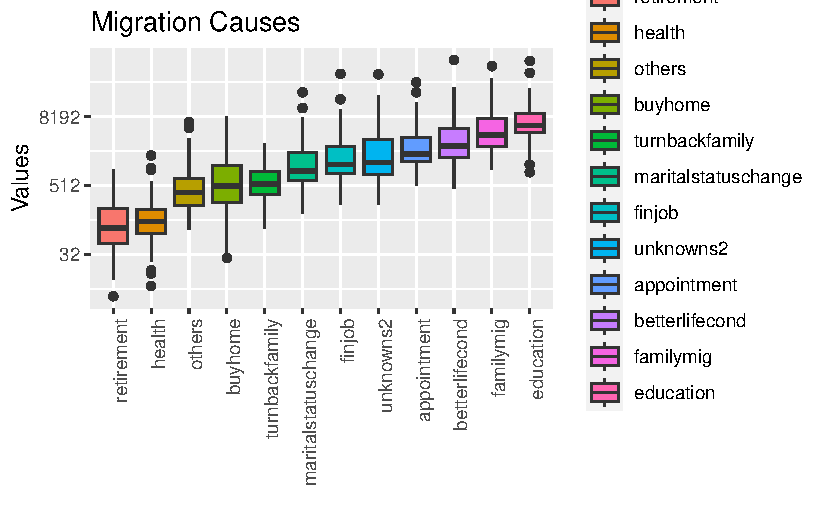
\includegraphics{analysis_files/figure-pdf/unnamed-chunk-2-1.pdf}

}

\end{figure}

To have an overview of data on migration causes we plotted a box plot to
see what reasons cause migration the most. Box plot shows that education
is the most common reason for migration followed by migration due to a
family member and better life conditions.

When plotting the box plot we scaled y values to log2 scale to see the
distribution better and we ordered the box plots to make it easier to
understand which are the most and the least causes of migration.

\hypertarget{regions-and-reasons-for-migration}{%
\subsection{Regions and Reasons for
Migration}\label{regions-and-reasons-for-migration}}

\begin{Shaded}
\begin{Highlighting}[]
\NormalTok{region\_plot }\OtherTok{\textless{}{-}}\NormalTok{ last\_migration\_tidy\_data }\SpecialCharTok{|\textgreater{}} \FunctionTok{select}\NormalTok{(migrationcauses,migrationcauses\_value,regions) }\SpecialCharTok{|\textgreater{}}
  \FunctionTok{ggplot}\NormalTok{(}\FunctionTok{aes}\NormalTok{(migrationcauses,migrationcauses\_value)) }\SpecialCharTok{+} \FunctionTok{geom\_point}\NormalTok{(}\FunctionTok{aes}\NormalTok{(}\AttributeTok{color =}\NormalTok{ regions)) }\SpecialCharTok{+}
  \FunctionTok{ggtitle}\NormalTok{(}\StringTok{"Regions and Reasons for Migration"}\NormalTok{) }\SpecialCharTok{+} \FunctionTok{xlab}\NormalTok{(}\StringTok{"Migration Causes"}\NormalTok{) }\SpecialCharTok{+}
  \FunctionTok{ylab}\NormalTok{(}\StringTok{"Migration Values"}\NormalTok{) }\SpecialCharTok{+} \FunctionTok{theme}\NormalTok{(}\AttributeTok{axis.text.x =} \FunctionTok{element\_text}\NormalTok{(}\AttributeTok{angle=} \DecValTok{90}\NormalTok{, }\AttributeTok{hjust =} \DecValTok{1}\NormalTok{)) }\SpecialCharTok{+} \FunctionTok{xlab}\NormalTok{(}\StringTok{""}\NormalTok{) }\SpecialCharTok{+} \FunctionTok{scale\_y\_continuous}\NormalTok{(}\AttributeTok{trans =} \StringTok{"log2"}\NormalTok{)  }
\FunctionTok{print}\NormalTok{(region\_plot)}
\end{Highlighting}
\end{Shaded}

\begin{figure}[H]

{\centering 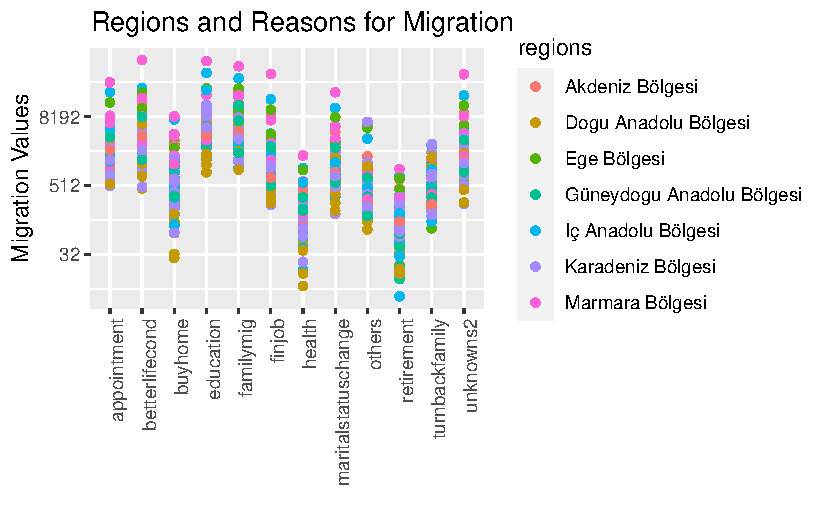
\includegraphics{analysis_files/figure-pdf/unnamed-chunk-3-1.pdf}

}

\end{figure}

When we analyze migration reasons on a regional basis, we observe that
under the category of `different reasons,' the highest migration has
occurred to the Marmara region. Following the Marmara region, the
second-highest migration took place to the Central Anatolia region. This
drew our attention to a few points. We had expected that the highest
migration due to retirement would be to the Central Anatolian Region or
Aegean Region, but it turned out that the majority of migration happened
to the Marmara region.

\hypertarget{metropolitan-cities-and-reasons-for-migration}{%
\subsection{Metropolitan Cities and Reasons for
Migration}\label{metropolitan-cities-and-reasons-for-migration}}

\begin{Shaded}
\begin{Highlighting}[]
\NormalTok{city\_plot }\OtherTok{\textless{}{-}}\NormalTok{ last\_migration\_tidy\_data }\SpecialCharTok{|\textgreater{}} \FunctionTok{filter}\NormalTok{(city }\SpecialCharTok{\%in\%} \FunctionTok{c}\NormalTok{(}\StringTok{"Ankara"}\NormalTok{,}\StringTok{"İstanbul"}\NormalTok{,}\StringTok{"İzmir"}\NormalTok{,}\StringTok{"Antalya"}\NormalTok{,}\StringTok{"Trabzon"}\NormalTok{,}\StringTok{"Ağrı"}\NormalTok{,}\StringTok{"Şanlıurfa"}\NormalTok{)) }\SpecialCharTok{|\textgreater{}} \FunctionTok{select}\NormalTok{(migrationcauses,migrationcauses\_value,city) }\SpecialCharTok{|\textgreater{}}
  \FunctionTok{ggplot}\NormalTok{(}\FunctionTok{aes}\NormalTok{(migrationcauses,migrationcauses\_value)) }\SpecialCharTok{+} \FunctionTok{geom\_point}\NormalTok{(}\FunctionTok{aes}\NormalTok{(}\AttributeTok{color =}\NormalTok{ city)) }\SpecialCharTok{+}
  \FunctionTok{ggtitle}\NormalTok{(}\StringTok{"Metropolitan Cities and Reasons for Migration"}\NormalTok{) }\SpecialCharTok{+} \FunctionTok{xlab}\NormalTok{(}\StringTok{"Migration Causes"}\NormalTok{) }\SpecialCharTok{+}
  \FunctionTok{ylab}\NormalTok{(}\StringTok{"Migration Values"}\NormalTok{) }\SpecialCharTok{+} \FunctionTok{theme}\NormalTok{(}\AttributeTok{axis.text.x =} \FunctionTok{element\_text}\NormalTok{(}\AttributeTok{angle=} \DecValTok{90}\NormalTok{, }\AttributeTok{hjust =} \DecValTok{1}\NormalTok{)) }\SpecialCharTok{+} \FunctionTok{xlab}\NormalTok{(}\StringTok{""}\NormalTok{) }\SpecialCharTok{+} \FunctionTok{scale\_y\_continuous}\NormalTok{(}\AttributeTok{trans =} \StringTok{"log2"}\NormalTok{)  }
\FunctionTok{print}\NormalTok{(city\_plot)}
\end{Highlighting}
\end{Shaded}

\begin{figure}[H]

{\centering 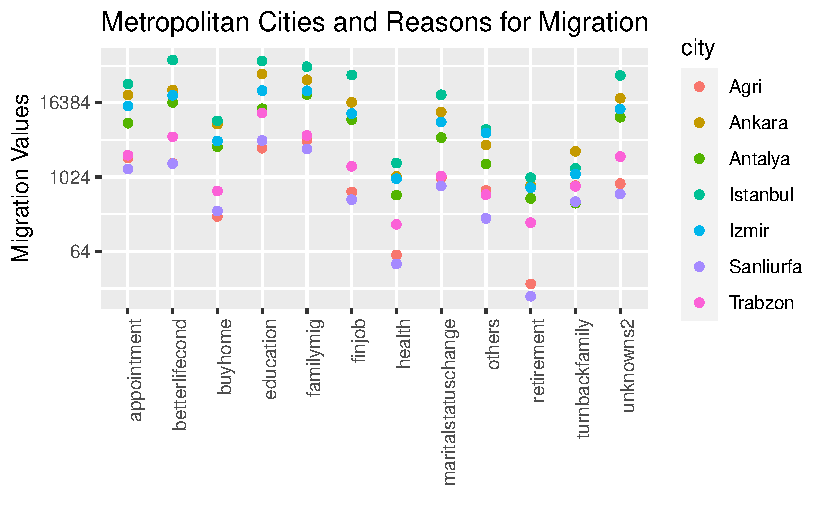
\includegraphics{analysis_files/figure-pdf/unnamed-chunk-4-1.pdf}

}

\end{figure}

While creating this graph, we included the most populous cities of each
region because plotting for all 81 provinces would be quite challenging.
As seen in this graph, the highest migration, due to different reasons,
has been to Istanbul, followed by Ankara. What surprised us again is
that the highest migration due to retirement is to İstanbul and
Ankara.''

\hypertarget{regions-and-migration-rates}{%
\subsection{Regions and Migration
Rates}\label{regions-and-migration-rates}}

\begin{Shaded}
\begin{Highlighting}[]
\NormalTok{migration\_gender2 }\OtherTok{\textless{}{-}}\NormalTok{ last\_migration\_tidy\_data }\SpecialCharTok{|\textgreater{}} \FunctionTok{mutate}\NormalTok{(}\AttributeTok{rate =}\NormalTok{ (last\_migration\_tidy\_data}\SpecialCharTok{$}\NormalTok{migrationcauses\_value) }\SpecialCharTok{/}\NormalTok{ (last\_migration\_tidy\_data}\SpecialCharTok{$}\NormalTok{gender\_value2))}

\NormalTok{region\_rate\_plot }\OtherTok{\textless{}{-}}\NormalTok{ migration\_gender2 }\SpecialCharTok{|\textgreater{}} \FunctionTok{ggplot}\NormalTok{(}\FunctionTok{aes}\NormalTok{(migrationcauses,rate)) }\SpecialCharTok{+} \FunctionTok{geom\_point}\NormalTok{(}\FunctionTok{aes}\NormalTok{(}\AttributeTok{color =}\NormalTok{ regions)) }\SpecialCharTok{+}
  \FunctionTok{ggtitle}\NormalTok{(}\StringTok{"Regions and Migration Rates"}\NormalTok{) }\SpecialCharTok{+} \FunctionTok{xlab}\NormalTok{(}\StringTok{"Migration Causes"}\NormalTok{) }\SpecialCharTok{+}
  \FunctionTok{ylab}\NormalTok{(}\StringTok{"Migration Rates"}\NormalTok{) }\SpecialCharTok{+} \FunctionTok{theme}\NormalTok{(}\AttributeTok{axis.text.x =} \FunctionTok{element\_text}\NormalTok{(}\AttributeTok{angle=} \DecValTok{45}\NormalTok{, }\AttributeTok{hjust =} \DecValTok{1}\NormalTok{)) }\SpecialCharTok{+} \FunctionTok{xlab}\NormalTok{(}\StringTok{""}\NormalTok{) }\SpecialCharTok{+} \FunctionTok{scale\_y\_continuous}\NormalTok{(}\AttributeTok{trans =} \StringTok{"log2"}\NormalTok{)}
  \FunctionTok{print}\NormalTok{(region\_rate\_plot)}
\end{Highlighting}
\end{Shaded}

\begin{figure}[H]

{\centering 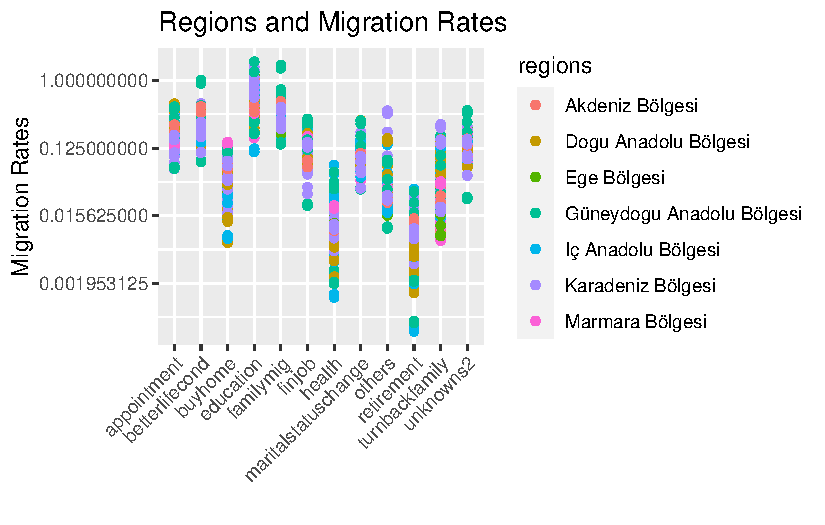
\includegraphics{analysis_files/figure-pdf/unnamed-chunk-5-1.pdf}

}

\end{figure}

In the above plots , plotted values were migration values with respect
to migration reason and we got some results that we were not expecting.
To understand the situation deeply we plotted migration rates rather
than migration values and result was more of what we were expected to
see. For example migration due to retirement was actually occurring to
Central Anatolian Region and Black Sea Region.

\hypertarget{metropolitan-cities-and-migration-rates}{%
\subsection{Metropolitan Cities and Migration
Rates}\label{metropolitan-cities-and-migration-rates}}

\begin{Shaded}
\begin{Highlighting}[]
\NormalTok{migration\_gender2 }\OtherTok{\textless{}{-}}\NormalTok{ last\_migration\_tidy\_data }\SpecialCharTok{|\textgreater{}} \FunctionTok{mutate}\NormalTok{(}\AttributeTok{rate =}\NormalTok{ (last\_migration\_tidy\_data}\SpecialCharTok{$}\NormalTok{migrationcauses\_value) }\SpecialCharTok{/}\NormalTok{ (last\_migration\_tidy\_data}\SpecialCharTok{$}\NormalTok{gender\_value2))}
\NormalTok{city\_rate\_plot }\OtherTok{\textless{}{-}}\NormalTok{ migration\_gender2 }\SpecialCharTok{|\textgreater{}} \FunctionTok{filter}\NormalTok{(city }\SpecialCharTok{\%in\%} \FunctionTok{c}\NormalTok{(}\StringTok{"Ankara"}\NormalTok{,}\StringTok{"İstanbul"}\NormalTok{,}\StringTok{"İzmir"}\NormalTok{,}\StringTok{"Antalya"}\NormalTok{,}\StringTok{"Trabzon"}\NormalTok{,}\StringTok{"Ağrı"}\NormalTok{,}\StringTok{"Şanlıurfa"}\NormalTok{)) }\SpecialCharTok{|\textgreater{}} \FunctionTok{ggplot}\NormalTok{(}\FunctionTok{aes}\NormalTok{(migrationcauses,rate)) }\SpecialCharTok{+} \FunctionTok{geom\_point}\NormalTok{(}\FunctionTok{aes}\NormalTok{(}\AttributeTok{color =}\NormalTok{ city)) }\SpecialCharTok{+}
    \FunctionTok{ggtitle}\NormalTok{(}\StringTok{"Metropolitan Cities and Migration Rates"}\NormalTok{) }\SpecialCharTok{+} \FunctionTok{xlab}\NormalTok{(}\StringTok{"Migration Causes"}\NormalTok{) }\SpecialCharTok{+}
    \FunctionTok{ylab}\NormalTok{(}\StringTok{"Migration Rates"}\NormalTok{) }\SpecialCharTok{+} \FunctionTok{theme}\NormalTok{(}\AttributeTok{axis.text.x =} \FunctionTok{element\_text}\NormalTok{(}\AttributeTok{angle=} \DecValTok{45}\NormalTok{, }\AttributeTok{hjust =} \DecValTok{1}\NormalTok{)) }\SpecialCharTok{+} \FunctionTok{xlab}\NormalTok{(}\StringTok{""}\NormalTok{) }\SpecialCharTok{+} \FunctionTok{scale\_y\_continuous}\NormalTok{(}\AttributeTok{trans =} \StringTok{"log2"}\NormalTok{)  }
  \FunctionTok{print}\NormalTok{(city\_rate\_plot) }
\end{Highlighting}
\end{Shaded}

\begin{figure}[H]

{\centering 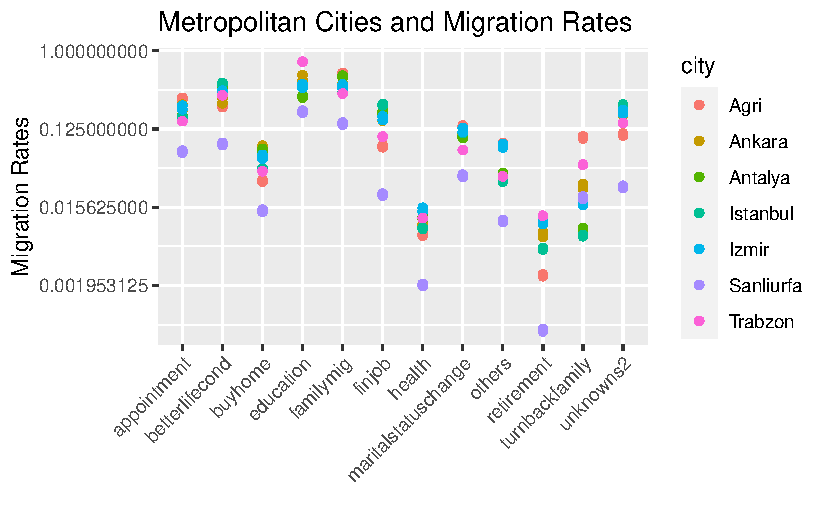
\includegraphics{analysis_files/figure-pdf/unnamed-chunk-6-1.pdf}

}

\end{figure}

In the same fashion, the city that people migrate the most due to
retirement is Trabzon followed by İzmir and Ankara.

\hypertarget{immigration-data-of-age-ranges}{%
\subsection{Immigration Data of Age
Ranges}\label{immigration-data-of-age-ranges}}

\begin{Shaded}
\begin{Highlighting}[]
\NormalTok{last\_migration\_tidy\_data }\SpecialCharTok{|\textgreater{}} \FunctionTok{mutate}\NormalTok{(}\AttributeTok{agerange2 =} \FunctionTok{reorder}\NormalTok{(agerange2, agerange\_value2, }\AttributeTok{FUN =}\NormalTok{ median)) }\SpecialCharTok{|\textgreater{}}
  \FunctionTok{ggplot}\NormalTok{(}\FunctionTok{aes}\NormalTok{(agerange2,agerange\_value2,}\AttributeTok{fill =}\NormalTok{ agerange2)) }\SpecialCharTok{+}
  \FunctionTok{geom\_boxplot}\NormalTok{() }\SpecialCharTok{+} \FunctionTok{ggtitle}\NormalTok{(}\StringTok{"Immigration Data of Age Ranges"}\NormalTok{) }\SpecialCharTok{+} \FunctionTok{xlab}\NormalTok{(}\StringTok{"Age Ranges"}\NormalTok{) }\SpecialCharTok{+}
  \FunctionTok{ylab}\NormalTok{(}\StringTok{"Values"}\NormalTok{) }\SpecialCharTok{+} \FunctionTok{theme}\NormalTok{(}\AttributeTok{axis.text.x =} \FunctionTok{element\_text}\NormalTok{(}\AttributeTok{angle=} \DecValTok{90}\NormalTok{, }\AttributeTok{hjust =} \DecValTok{1}\NormalTok{)) }\SpecialCharTok{+} \FunctionTok{xlab}\NormalTok{(}\StringTok{""}\NormalTok{) }\SpecialCharTok{+}
  \FunctionTok{scale\_y\_continuous}\NormalTok{(}\AttributeTok{trans =} \StringTok{"log2"}\NormalTok{) }
\end{Highlighting}
\end{Shaded}

\begin{figure}[H]

{\centering 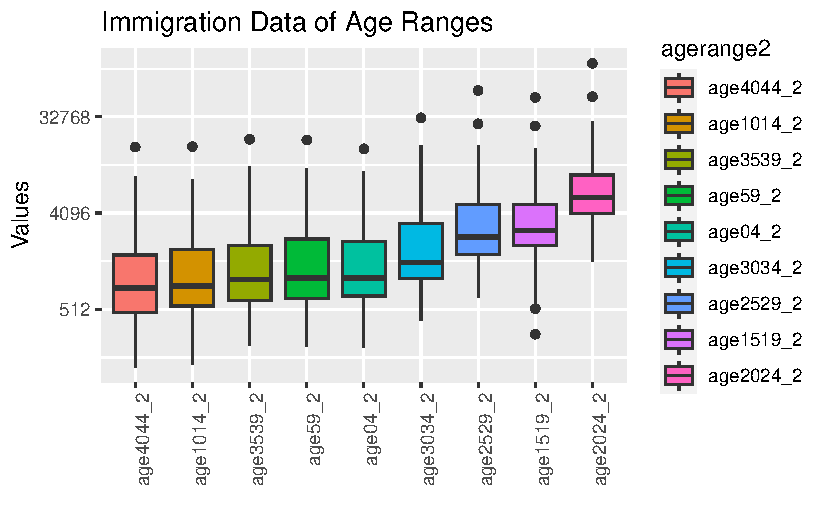
\includegraphics{analysis_files/figure-pdf/unnamed-chunk-7-1.pdf}

}

\end{figure}

When we look at the graph, we see that the age range of the people who
migrate the most is 20-24. The 15-19 age range ranks second. The age
range of people who migrate the least is observed to be 40-44. When we
look at the Immigration Data of Age Ranges, we see that the most
immigration age range is 20-24. We can say that education was the
highest value among the reasons for immigration and this is consistent
with this. Likewise, the second place is 15-19. It can be interpreted
that high school students also migrate for education. ``finjob'' ranks
in the middle list of reasons for migration. If we consider 25-29 as the
age for finding a job, we can comment that people aged 25-29 do not
migrate only for the purpose of finding a job. For example, they may
have migrated due to better living conditions. When we look at the
graph, we see that the migration age of 40-44 migrates the least
compared to other ages. In our opinion, we can conclude from the graph
that people who are used to a certain order no longer want change.
According to the chart, 10-14 years old is the second to last migration
age range. ``familymig'' ranked second among the reasons for migration.
We can say that there is a contradiction here. We would have expected a
higher number of people migrating for health reasons. Health is very
important for everyone, but unfortunately health services are not
developed everywhere. Health problems are a factor that can be seen in
all age groups, so we would expect the values to be high.

\hypertarget{correlations-between-migration-reasons-and-age-ranges.}{%
\subsection{Correlations Between Migration Reasons and Age
Ranges.}\label{correlations-between-migration-reasons-and-age-ranges.}}

\begin{Shaded}
\begin{Highlighting}[]
\FunctionTok{cor}\NormalTok{(last\_migration\_tidy\_data}\SpecialCharTok{$}\NormalTok{migrationcauses\_value, last\_migration\_tidy\_data}\SpecialCharTok{$}\NormalTok{agerange\_value2)}
\end{Highlighting}
\end{Shaded}

\begin{verbatim}
[1] 0.4977804
\end{verbatim}

This value indicates a moderate positive relationship between migration
reasons and age ranges.

\hypertarget{education-level-and-fertility-rate-in-geographical-regions}{%
\subsection{Education Level and Fertility Rate in Geographical
Regions}\label{education-level-and-fertility-rate-in-geographical-regions}}

\begin{Shaded}
\begin{Highlighting}[]
\FunctionTok{library}\NormalTok{(tidyverse)}
\CommentTok{\# Extracting necessary columns from the \textquotesingle{}last\_tidy\_data\_education2\textquotesingle{} dataset}
\NormalTok{data }\OtherTok{\textless{}{-}}\NormalTok{ last\_tidy\_data\_education2 }\SpecialCharTok{\%\textgreater{}\%}
  \FunctionTok{select}\NormalTok{(regions, education, education\_value, fertilityrate) }
\CommentTok{\# Calculating average education and fertility rate per region}
\NormalTok{education\_fertility }\OtherTok{\textless{}{-}}\NormalTok{ data }\SpecialCharTok{\%\textgreater{}\%}
  \FunctionTok{group\_by}\NormalTok{(regions) }\SpecialCharTok{\%\textgreater{}\%}
  \FunctionTok{summarise}\NormalTok{(}
    \AttributeTok{avg\_education =} \FunctionTok{mean}\NormalTok{(education\_value),  }\CommentTok{\# Calculating the mean education value for each region}
    \AttributeTok{avg\_fertility =} \FunctionTok{mean}\NormalTok{(fertilityrate)     }\CommentTok{\# Calculating the mean fertility rate for each region}
\NormalTok{  )}
\CommentTok{\# Creating a scatter plot to visualize the relationship between education level and fertility rate across regions}
\FunctionTok{ggplot}\NormalTok{(education\_fertility, }\FunctionTok{aes}\NormalTok{(}\AttributeTok{x =}\NormalTok{ avg\_education, }\AttributeTok{y =}\NormalTok{ avg\_fertility, }\AttributeTok{label =}\NormalTok{ regions)) }\SpecialCharTok{+}
  \FunctionTok{geom\_point}\NormalTok{(}\AttributeTok{color =} \StringTok{"blue"}\NormalTok{) }\SpecialCharTok{+}  \CommentTok{\# Adding points to represent each region}
  \FunctionTok{geom\_text}\NormalTok{(}\AttributeTok{hjust =} \DecValTok{0}\NormalTok{, }\AttributeTok{vjust =} \DecValTok{0}\NormalTok{, }\AttributeTok{size =} \DecValTok{3}\NormalTok{, }\AttributeTok{color =} \StringTok{"black"}\NormalTok{, }\AttributeTok{alpha =} \FloatTok{0.8}\NormalTok{) }\SpecialCharTok{+}  \CommentTok{\# Adding text labels for regions}
  \FunctionTok{labs}\NormalTok{(}
    \AttributeTok{title =} \StringTok{"Education Level and Fertility Rate in Geographical Regions"}\NormalTok{,  }\CommentTok{\# Title of the plot}
    \AttributeTok{x =} \StringTok{"Average Education Level"}\NormalTok{,  }\CommentTok{\# X{-}axis label}
    \AttributeTok{y =} \StringTok{"Average Fertility Rate"}     \CommentTok{\# Y{-}axis label}
\NormalTok{  ) }\SpecialCharTok{+}
  \FunctionTok{scale\_x\_continuous}\NormalTok{(}\AttributeTok{labels =}\NormalTok{ scales}\SpecialCharTok{::}\NormalTok{comma, }\AttributeTok{breaks =} \FunctionTok{seq}\NormalTok{(}\DecValTok{0}\NormalTok{, }\DecValTok{300000}\NormalTok{, }\AttributeTok{by =} \DecValTok{50000}\NormalTok{))  }\CommentTok{\# Formatting X{-}axis labels}
\end{Highlighting}
\end{Shaded}

\begin{figure}[H]

{\centering 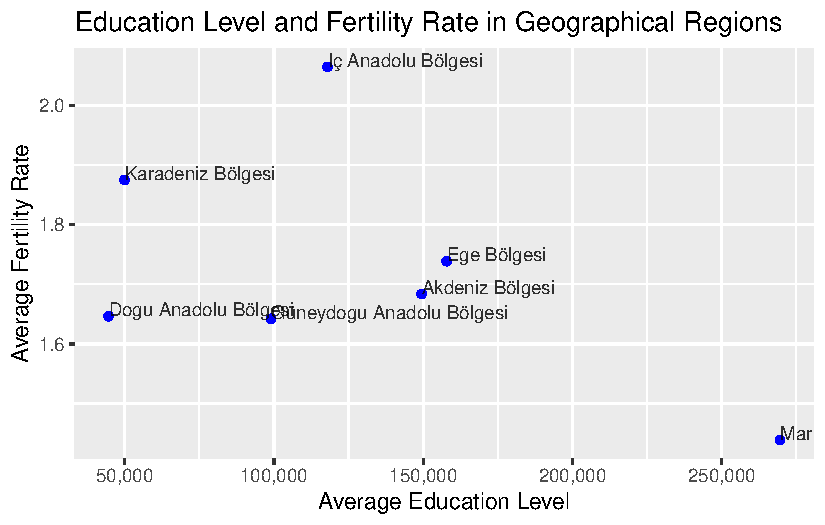
\includegraphics{analysis_files/figure-pdf/unnamed-chunk-9-1.pdf}

}

\end{figure}

The scatter plot does not show a clear correlation between the average
education level and fertility rate across regions. The points
representing different regions are scattered without showing a clear
trend of increase or decrease. The region with the highest average
education level is Marmara, with about 250,000 units of education value.
The region with the lowest average education level is Eastern Anatolia
Region, with about 50,000 units of education value. The region with the
highest average fertility rate is Central Anatolia Region, with above
2.0 children per woman. The region with the lowest average fertility
rate is the Marmara Region, with below 1.5 children per woman. There are
some outliers in the data, such as Central Anatolia Region, which has a
relatively high average education level but also a high average
fertility rate, and Mediterranean Region, which has a relatively low
average education level but also a low average fertility rate. These
outliers may indicate that there are other factors influencing the
fertility rate besides the education level, such as culture, religion,
income, etc. The surprising point in this data is that I expected the
Eastern Anatolia Region to have the highest fertility rate. The low
population registration rates in that region may be one of the reasons
affecting the data output. According to TUIK data, the population
registration rate of the Eastern Anatolia Region is 97.92\%, which is
98.82\% below the Turkey average. This may mean that some of the
children born in this region are not registered.

\hypertarget{migration-distribution-by-education-levels-for-26-regions}{%
\subsection{Migration Distribution by Education Levels for 26
Regions}\label{migration-distribution-by-education-levels-for-26-regions}}

\begin{Shaded}
\begin{Highlighting}[]
\FunctionTok{library}\NormalTok{(tidyverse)}
\CommentTok{\# Merging population and migration datasets based on the \textquotesingle{}city\textquotesingle{} column}
\NormalTok{merged\_data }\OtherTok{\textless{}{-}}\NormalTok{ population }\SpecialCharTok{\%\textgreater{}\%}
  \FunctionTok{inner\_join}\NormalTok{(migration, }\AttributeTok{by =} \StringTok{"city"}\NormalTok{) }\SpecialCharTok{\%\textgreater{}\%}
  \CommentTok{\# Selecting specific columns from the merged dataset}
  \FunctionTok{select}\NormalTok{(city, region2id, university2, highschool2, middleschool2, elementaryschool2)}

\CommentTok{\# Transforming the merged data into a tidy format using pivot\_longer}
\NormalTok{merged\_data\_tidy }\OtherTok{\textless{}{-}}\NormalTok{ merged\_data }\SpecialCharTok{\%\textgreater{}\%}
  \FunctionTok{pivot\_longer}\NormalTok{(}
    \AttributeTok{cols =} \FunctionTok{c}\NormalTok{(university2, highschool2, middleschool2, elementaryschool2),}
    \AttributeTok{names\_to =} \StringTok{"education\_level"}\NormalTok{,}
    \AttributeTok{values\_to =} \StringTok{"migration\_count"}
\NormalTok{  ) }\SpecialCharTok{\%\textgreater{}\%}
  \CommentTok{\# Grouping by region and education level to calculate total migration counts}
  \FunctionTok{group\_by}\NormalTok{(region2id, education\_level) }\SpecialCharTok{\%\textgreater{}\%}
  \FunctionTok{summarise}\NormalTok{(}\AttributeTok{total\_migration =} \FunctionTok{sum}\NormalTok{(migration\_count, }\AttributeTok{na.rm =} \ConstantTok{TRUE}\NormalTok{)) }\SpecialCharTok{\%\textgreater{}\%}
  \FunctionTok{ungroup}\NormalTok{() }\SpecialCharTok{\%\textgreater{}\%}
  \CommentTok{\# Renaming education levels for better readability}
  \FunctionTok{mutate}\NormalTok{(}
    \AttributeTok{education\_level =} \FunctionTok{case\_when}\NormalTok{(}
\NormalTok{      education\_level }\SpecialCharTok{==} \StringTok{"university2"} \SpecialCharTok{\textasciitilde{}} \StringTok{"University"}\NormalTok{,}
\NormalTok{      education\_level }\SpecialCharTok{==} \StringTok{"middleschool2"} \SpecialCharTok{\textasciitilde{}} \StringTok{"Middle School"}\NormalTok{,}
\NormalTok{      education\_level }\SpecialCharTok{==} \StringTok{"highschool2"} \SpecialCharTok{\textasciitilde{}} \StringTok{"High School"}\NormalTok{,}
\NormalTok{      education\_level }\SpecialCharTok{==} \StringTok{"elementaryschool2"} \SpecialCharTok{\textasciitilde{}} \StringTok{"Elementary School"}\NormalTok{,}
      \ConstantTok{TRUE} \SpecialCharTok{\textasciitilde{}} \FunctionTok{as.character}\NormalTok{(education\_level)}
\NormalTok{    )}
\NormalTok{  )  }

\CommentTok{\# Sorting regions based on total migration counts}
\NormalTok{sorted\_regions }\OtherTok{\textless{}{-}}\NormalTok{ merged\_data\_tidy }\SpecialCharTok{\%\textgreater{}\%}
  \FunctionTok{group\_by}\NormalTok{(region2id) }\SpecialCharTok{\%\textgreater{}\%}
  \FunctionTok{summarise}\NormalTok{(}\AttributeTok{total\_migration =} \FunctionTok{sum}\NormalTok{(total\_migration, }\AttributeTok{na.rm =} \ConstantTok{TRUE}\NormalTok{)) }\SpecialCharTok{\%\textgreater{}\%}
  \FunctionTok{arrange}\NormalTok{(}\FunctionTok{desc}\NormalTok{(total\_migration)) }\SpecialCharTok{\%\textgreater{}\%} 
  \FunctionTok{pull}\NormalTok{(region2id)}

\CommentTok{\# Reordering factor levels of \textquotesingle{}region2id\textquotesingle{} based on sorted regions}
\NormalTok{merged\_data\_tidy}\SpecialCharTok{$}\NormalTok{region2id }\OtherTok{\textless{}{-}} \FunctionTok{factor}\NormalTok{(merged\_data\_tidy}\SpecialCharTok{$}\NormalTok{region2id, }\AttributeTok{levels =}\NormalTok{ sorted\_regions)}

\CommentTok{\# Creating a stacked bar plot to visualize migration distribution by education levels across regions}
\FunctionTok{ggplot}\NormalTok{(merged\_data\_tidy, }\FunctionTok{aes}\NormalTok{(}\AttributeTok{x =}\NormalTok{ region2id, }\AttributeTok{y =}\NormalTok{ total\_migration, }\AttributeTok{fill =}\NormalTok{ education\_level)) }\SpecialCharTok{+}
  \FunctionTok{geom\_bar}\NormalTok{(}\AttributeTok{stat =} \StringTok{"identity"}\NormalTok{, }\AttributeTok{position =} \StringTok{"stack"}\NormalTok{) }\SpecialCharTok{+}  \CommentTok{\# Stacked bar plot}
  \FunctionTok{labs}\NormalTok{(}
    \AttributeTok{title =} \StringTok{"Migration Distribution by Education Levels for 26 Regions"}\NormalTok{,  }\CommentTok{\# Title of the plot}
    \AttributeTok{x =} \StringTok{"Regions"}\NormalTok{,  }\CommentTok{\# X{-}axis label}
    \AttributeTok{y =} \StringTok{"Number of People Immigrating"}\NormalTok{,  }\CommentTok{\# Y{-}axis label}
    \AttributeTok{fill =} \StringTok{"Education Levels"}  \CommentTok{\# Legend label}
\NormalTok{  ) }\SpecialCharTok{+}
  \FunctionTok{theme}\NormalTok{(}\AttributeTok{axis.text.x =} \FunctionTok{element\_text}\NormalTok{(}\AttributeTok{angle =} \DecValTok{45}\NormalTok{, }\AttributeTok{hjust =} \DecValTok{1}\NormalTok{)) }\SpecialCharTok{+}  \CommentTok{\# Rotating x{-}axis labels for better readability}
  \FunctionTok{scale\_fill\_brewer}\NormalTok{(}\AttributeTok{palette =} \StringTok{"Set3"}\NormalTok{) }\SpecialCharTok{+}  \CommentTok{\# Setting color palette for education levels}
  \FunctionTok{scale\_y\_continuous}\NormalTok{(}\AttributeTok{labels =}\NormalTok{ scales}\SpecialCharTok{::}\NormalTok{comma)  }\CommentTok{\# Formatting Y{-}axis labels using commas for better readability}
\end{Highlighting}
\end{Shaded}

\begin{figure}[H]

{\centering 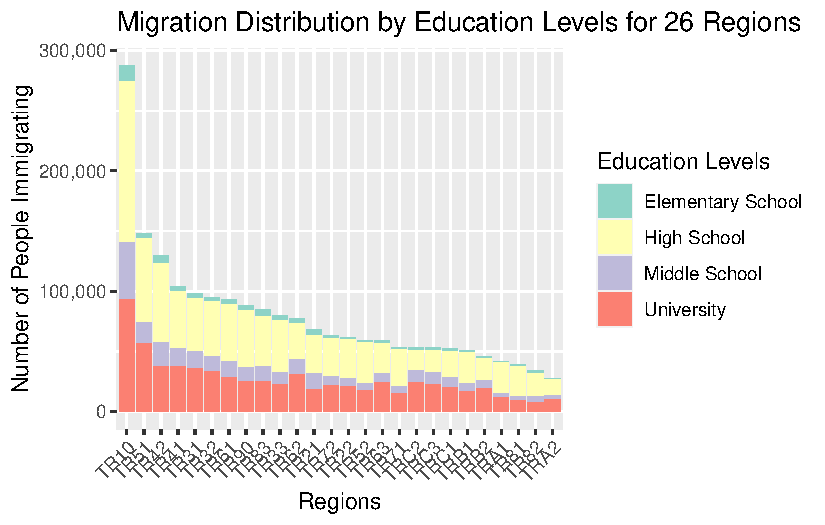
\includegraphics{analysis_files/figure-pdf/unnamed-chunk-10-1.pdf}

}

\end{figure}

It is seen that immigrants with high education levels mostly migrate to
regions numbered TR10, TR51 and TR42. These regions cover the
northwestern, western and southwestern regions of Turkey. It may
indicate that these regions are more attractive in terms of education
and job opportunities. It is seen that immigrants with low education
level mostly migrate to TR81, TR82 and TRA2 regions. These regions cover
the northeastern, eastern and southeastern regions of Turkey. It may
indicate that these regions are poorer in terms of education and job
opportunities. It may indicate that other Regions are average in terms
of education and job opportunities.

\hypertarget{migration-by-education-level}{%
\subsection{Migration by Education
Level}\label{migration-by-education-level}}

\begin{Shaded}
\begin{Highlighting}[]
\FunctionTok{library}\NormalTok{(tidyverse)}

\CommentTok{\# Merging two datasets \textquotesingle{}population\textquotesingle{} and \textquotesingle{}migration\textquotesingle{} based on the common column \textquotesingle{}city\textquotesingle{}}
\NormalTok{merged\_data }\OtherTok{\textless{}{-}} \FunctionTok{inner\_join}\NormalTok{(population, migration, }\AttributeTok{by =} \StringTok{"city"}\NormalTok{) }\SpecialCharTok{\%\textgreater{}\%}
  \CommentTok{\# Selecting specific columns from the merged dataset}
  \FunctionTok{select}\NormalTok{(city, region2id, university2, doctorate, highschool2, elementaryschool2, middleschool2, finjob)}

\CommentTok{\# Reshaping the data using pivot\_longer to gather migration counts for different education levels}
\NormalTok{education\_migration }\OtherTok{\textless{}{-}}\NormalTok{ merged\_data }\SpecialCharTok{\%\textgreater{}\%}
  \FunctionTok{pivot\_longer}\NormalTok{(}
    \AttributeTok{cols =} \FunctionTok{c}\NormalTok{(university2, doctorate, highschool2, elementaryschool2, middleschool2),}
    \AttributeTok{names\_to =} \StringTok{"education\_level"}\NormalTok{,}
    \AttributeTok{values\_to =} \StringTok{"migration\_count"}
\NormalTok{  ) }\SpecialCharTok{\%\textgreater{}\%}
  \CommentTok{\# Renaming and categorizing education levels for better visualization}
  \FunctionTok{mutate}\NormalTok{(}
    \AttributeTok{education\_level =} \FunctionTok{case\_when}\NormalTok{(}
\NormalTok{      education\_level }\SpecialCharTok{==} \StringTok{"university2"} \SpecialCharTok{\textasciitilde{}} \StringTok{"University"}\NormalTok{,}
\NormalTok{      education\_level }\SpecialCharTok{==} \StringTok{"doctorate"} \SpecialCharTok{\textasciitilde{}} \StringTok{"Doctorate"}\NormalTok{,}
\NormalTok{      education\_level }\SpecialCharTok{==} \StringTok{"highschool2"} \SpecialCharTok{\textasciitilde{}} \StringTok{"High School"}\NormalTok{,}
\NormalTok{      education\_level }\SpecialCharTok{==} \StringTok{"elementaryschool2"} \SpecialCharTok{\textasciitilde{}} \StringTok{"Elementary School"}\NormalTok{,}
\NormalTok{      education\_level }\SpecialCharTok{==} \StringTok{"middleschool2"} \SpecialCharTok{\textasciitilde{}} \StringTok{"Middle School"}\NormalTok{,}
      \ConstantTok{TRUE} \SpecialCharTok{\textasciitilde{}} \FunctionTok{as.character}\NormalTok{(education\_level)}
\NormalTok{    )}
\NormalTok{  )}

\CommentTok{\# Setting the order of the education levels for better visualization}
\NormalTok{education\_migration}\SpecialCharTok{$}\NormalTok{education\_level }\OtherTok{\textless{}{-}} \FunctionTok{factor}\NormalTok{(education\_migration}\SpecialCharTok{$}\NormalTok{education\_level, }
                                             \AttributeTok{levels =} \FunctionTok{c}\NormalTok{(}\StringTok{"Elementary School"}\NormalTok{, }\StringTok{"Middle School"}\NormalTok{, }\StringTok{"High School"}\NormalTok{, }\StringTok{"University"}\NormalTok{, }\StringTok{"Doctorate"}\NormalTok{))}

\CommentTok{\# Creating a boxplot to visualize the migration count across different education levels}
\FunctionTok{ggplot}\NormalTok{(education\_migration, }\FunctionTok{aes}\NormalTok{(}\AttributeTok{x =}\NormalTok{ education\_level, }\AttributeTok{y =}\NormalTok{ migration\_count, }\AttributeTok{fill =}\NormalTok{ education\_level)) }\SpecialCharTok{+}
  \FunctionTok{geom\_boxplot}\NormalTok{() }\SpecialCharTok{+}  \CommentTok{\# Adding boxplot geometry}
  \FunctionTok{labs}\NormalTok{(}
    \AttributeTok{title =} \StringTok{"Migration by Education Level"}\NormalTok{,  }\CommentTok{\# Title of the plot}
    \AttributeTok{x =} \StringTok{"Education Level"}\NormalTok{,  }\CommentTok{\# X{-}axis label}
    \AttributeTok{y =} \StringTok{"Migration Count"}\NormalTok{,  }\CommentTok{\# Y{-}axis label}
    \AttributeTok{fill =} \StringTok{"Education Level"}  \CommentTok{\# Legend label}
\NormalTok{  ) }\SpecialCharTok{+}
  \FunctionTok{theme\_minimal}\NormalTok{() }\SpecialCharTok{+}  \CommentTok{\# Applying a minimal theme to the plot}
  \FunctionTok{scale\_y\_continuous}\NormalTok{(}\AttributeTok{labels =}\NormalTok{ scales}\SpecialCharTok{::}\NormalTok{comma)  }\CommentTok{\# Formatting Y{-}axis labels with commas for thousands}
\end{Highlighting}
\end{Shaded}

\begin{figure}[H]

{\centering 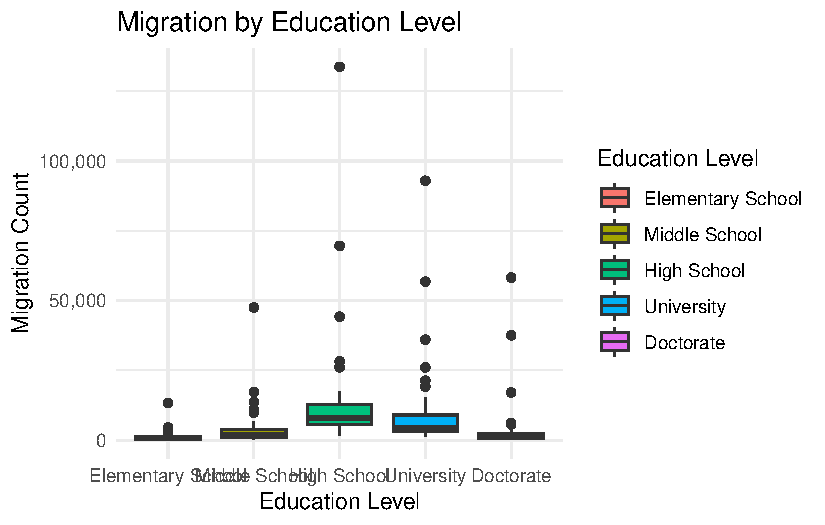
\includegraphics{analysis_files/figure-pdf/unnamed-chunk-11-1.pdf}

}

\end{figure}

On the x axis, there are four education levels: doctorate, primary
school, high school and university. On the Y axis, the number of people
migrating is shown with values ranging from 0 to 100,000. In the graph,
the number of migrations of individuals at doctoral or primary school
level is much less than that of individuals at high school and
university levels. In the graph, the highest number of migrations is
seen among individuals at university level. This is followed by
individuals at the high school level. It is seen that individuals with a
higher level of education migrate less than individuals with a lower
level of education. This may indicate that individuals with higher
levels of education are more dependent on working conditions or find
fewer job opportunities. It is seen that individuals with low education
levels migrate more than individuals with high education levels. This
may indicate that individuals with lower levels of education strive more
to improve their living conditions or are under more pressure.

\hypertarget{inter-regional-rate-distributions}{%
\subsection{Inter-regional Rate
Distributions}\label{inter-regional-rate-distributions}}

\begin{Shaded}
\begin{Highlighting}[]
\NormalTok{migration\_rate }\OtherTok{\textless{}{-}}\NormalTok{ (migration}\SpecialCharTok{$}\NormalTok{male2}\SpecialCharTok{+}\NormalTok{migration}\SpecialCharTok{$}\NormalTok{female2)}\SpecialCharTok{/}\NormalTok{population}\SpecialCharTok{$}\NormalTok{totalpop}
\NormalTok{numberofattempts\_rate }\OtherTok{\textless{}{-}}\NormalTok{ population}\SpecialCharTok{$}\NormalTok{numberofattempts}\SpecialCharTok{/}\NormalTok{population}\SpecialCharTok{$}\NormalTok{totalpop}
\NormalTok{housingsalesnumbers\_rate }\OtherTok{\textless{}{-}}\NormalTok{ population}\SpecialCharTok{$}\NormalTok{housingsalesnumbers}\SpecialCharTok{/}\NormalTok{population}\SpecialCharTok{$}\NormalTok{totalpop}
\NormalTok{electricity\_rate }\OtherTok{\textless{}{-}}\NormalTok{ population}\SpecialCharTok{$}\NormalTok{electricity}\SpecialCharTok{/}\NormalTok{population}\SpecialCharTok{$}\NormalTok{totalpop}
\NormalTok{educated\_rate }\OtherTok{\textless{}{-}}\NormalTok{ (population}\SpecialCharTok{$}\NormalTok{highschool }\SpecialCharTok{+}\NormalTok{ population}\SpecialCharTok{$}\NormalTok{university }\SpecialCharTok{+}\NormalTok{ population}\SpecialCharTok{$}\NormalTok{master }\SpecialCharTok{+}\NormalTok{ population}\SpecialCharTok{$}\NormalTok{doctorate)}\SpecialCharTok{/}\NormalTok{population}\SpecialCharTok{$}\NormalTok{totalpop}

\NormalTok{merged\_data }\OtherTok{\textless{}{-}} \FunctionTok{cbind}\NormalTok{(population, numberofattempts\_rate, housingsalesnumbers\_rate, electricity\_rate)}

\NormalTok{merged\_data}\SpecialCharTok{$}\NormalTok{regions }\OtherTok{\textless{}{-}} \FunctionTok{factor}\NormalTok{(merged\_data}\SpecialCharTok{$}\NormalTok{regions) }




\NormalTok{merged\_data\_long }\OtherTok{\textless{}{-}}\NormalTok{ merged\_data }\SpecialCharTok{\%\textgreater{}\%}
  \FunctionTok{pivot\_longer}\NormalTok{(}\AttributeTok{cols =} \FunctionTok{c}\NormalTok{(numberofattempts\_rate, housingsalesnumbers\_rate, electricity\_rate),}
               \AttributeTok{names\_to =} \StringTok{"variable"}\NormalTok{, }\AttributeTok{values\_to =} \StringTok{"rate"}\NormalTok{)}


\FunctionTok{ggplot}\NormalTok{(merged\_data\_long, }\FunctionTok{aes}\NormalTok{(}\AttributeTok{x =}\NormalTok{ regions, }\AttributeTok{y =}\NormalTok{ rate, }\AttributeTok{fill =}\NormalTok{ regions)) }\SpecialCharTok{+}
  \FunctionTok{geom\_boxplot}\NormalTok{() }\SpecialCharTok{+}
  \FunctionTok{labs}\NormalTok{(}\AttributeTok{x =} \StringTok{"Regions"}\NormalTok{, }\AttributeTok{y =} \StringTok{"Rate"}\NormalTok{, }\AttributeTok{title =} \StringTok{"Interregional Rate Distributions"}\NormalTok{) }\SpecialCharTok{+}
  \FunctionTok{facet\_wrap}\NormalTok{(}\SpecialCharTok{\textasciitilde{}}\NormalTok{ variable, }\AttributeTok{scales =} \StringTok{"free\_y"}\NormalTok{, }\AttributeTok{ncol =} \DecValTok{1}\NormalTok{) }\SpecialCharTok{+}
  \FunctionTok{theme}\NormalTok{(}\AttributeTok{axis.text.x =} \FunctionTok{element\_text}\NormalTok{(}\AttributeTok{angle =} \DecValTok{45}\NormalTok{, }\AttributeTok{hjust =} \DecValTok{1}\NormalTok{))}
\end{Highlighting}
\end{Shaded}

\begin{figure}[H]

{\centering 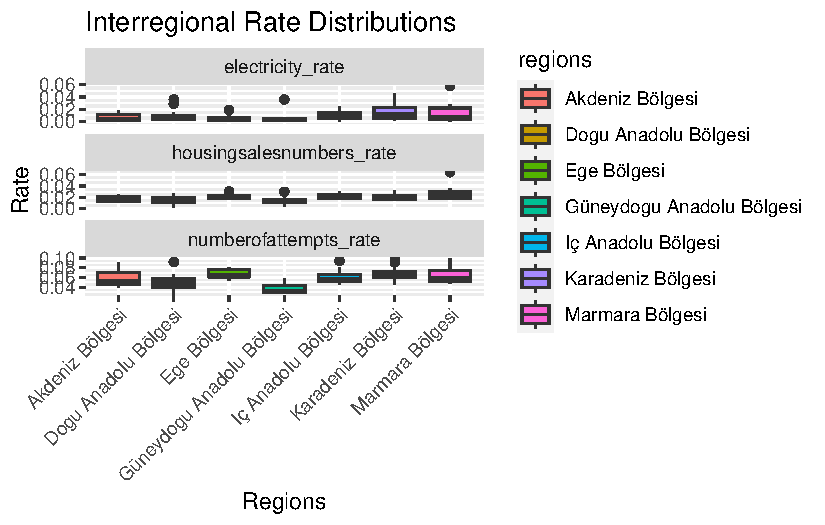
\includegraphics{analysis_files/figure-pdf/unnamed-chunk-12-1.pdf}

}

\end{figure}

\begin{Shaded}
\begin{Highlighting}[]
\NormalTok{ratios }\OtherTok{\textless{}{-}} \FunctionTok{data.frame}\NormalTok{(}
\NormalTok{  electricity\_rate ,  }
\NormalTok{ housingsalesnumbers\_rate,}
\NormalTok{  numberofattempts\_rate,}
\NormalTok{  migration\_rate,}
\NormalTok{ educated\_rate}
\NormalTok{)}

\NormalTok{correlation\_matrix }\OtherTok{\textless{}{-}} \FunctionTok{cor}\NormalTok{(ratios)}

\FunctionTok{print}\NormalTok{(correlation\_matrix)}
\end{Highlighting}
\end{Shaded}

\begin{verbatim}
                         electricity_rate housingsalesnumbers_rate
electricity_rate                1.0000000                0.2673481
housingsalesnumbers_rate        0.2673481                1.0000000
numberofattempts_rate           0.4605411                0.4822953
migration_rate                  0.6837392                0.2184274
educated_rate                   0.6228220                0.2711951
                         numberofattempts_rate migration_rate educated_rate
electricity_rate                     0.4605411      0.6837392     0.6228220
housingsalesnumbers_rate             0.4822953      0.2184274     0.2711951
numberofattempts_rate                1.0000000      0.5059387     0.6996717
migration_rate                       0.5059387      1.0000000     0.8014049
educated_rate                        0.6996717      0.8014049     1.0000000
\end{verbatim}

\begin{Shaded}
\begin{Highlighting}[]
\NormalTok{population}\SpecialCharTok{$}\StringTok{\textasciigrave{}}\AttributeTok{Migration Rate}\StringTok{\textasciigrave{}} \OtherTok{\textless{}{-}}\NormalTok{ (migration}\SpecialCharTok{$}\NormalTok{male2 }\SpecialCharTok{+}\NormalTok{ migration}\SpecialCharTok{$}\NormalTok{female2) }\SpecialCharTok{/}\NormalTok{ population}\SpecialCharTok{$}\NormalTok{totalpop}
\NormalTok{population}\SpecialCharTok{$}\StringTok{\textasciigrave{}}\AttributeTok{Number of Attempts Rate}\StringTok{\textasciigrave{}} \OtherTok{\textless{}{-}}\NormalTok{ population}\SpecialCharTok{$}\NormalTok{numberofattempts }\SpecialCharTok{/}\NormalTok{ population}\SpecialCharTok{$}\NormalTok{totalpop}
\NormalTok{population}\SpecialCharTok{$}\StringTok{\textasciigrave{}}\AttributeTok{Housing Sales Numbers Rate}\StringTok{\textasciigrave{}} \OtherTok{\textless{}{-}}\NormalTok{ population}\SpecialCharTok{$}\NormalTok{housingsalesnumbers }\SpecialCharTok{/}\NormalTok{ population}\SpecialCharTok{$}\NormalTok{totalpop}
\NormalTok{population}\SpecialCharTok{$}\StringTok{\textasciigrave{}}\AttributeTok{Electricity Rate}\StringTok{\textasciigrave{}} \OtherTok{\textless{}{-}}\NormalTok{ population}\SpecialCharTok{$}\NormalTok{electricity }\SpecialCharTok{/}\NormalTok{ population}\SpecialCharTok{$}\NormalTok{totalpop}


\NormalTok{rates\_data }\OtherTok{\textless{}{-}}\NormalTok{ population }\SpecialCharTok{\%\textgreater{}\%}
  \FunctionTok{select}\NormalTok{(city, region2id, }\StringTok{\textasciigrave{}}\AttributeTok{Migration Rate}\StringTok{\textasciigrave{}}\NormalTok{, }\StringTok{\textasciigrave{}}\AttributeTok{Number of Attempts Rate}\StringTok{\textasciigrave{}}\NormalTok{, }\StringTok{\textasciigrave{}}\AttributeTok{Housing Sales Numbers Rate}\StringTok{\textasciigrave{}}\NormalTok{, }\StringTok{\textasciigrave{}}\AttributeTok{Electricity Rate}\StringTok{\textasciigrave{}}\NormalTok{)}

\NormalTok{rates\_data\_tidy }\OtherTok{\textless{}{-}}\NormalTok{ rates\_data }\SpecialCharTok{\%\textgreater{}\%}
  \FunctionTok{pivot\_longer}\NormalTok{(}
    \AttributeTok{cols =} \FunctionTok{c}\NormalTok{(}\StringTok{\textasciigrave{}}\AttributeTok{Migration Rate}\StringTok{\textasciigrave{}}\NormalTok{, }\StringTok{\textasciigrave{}}\AttributeTok{Number of Attempts Rate}\StringTok{\textasciigrave{}}\NormalTok{, }\StringTok{\textasciigrave{}}\AttributeTok{Housing Sales Numbers Rate}\StringTok{\textasciigrave{}}\NormalTok{, }\StringTok{\textasciigrave{}}\AttributeTok{Electricity Rate}\StringTok{\textasciigrave{}}\NormalTok{),}
    \AttributeTok{names\_to =} \StringTok{"rate\_type"}\NormalTok{,}
    \AttributeTok{values\_to =} \StringTok{"rate\_value"}
\NormalTok{  )}

\FunctionTok{ggplot}\NormalTok{(rates\_data\_tidy, }\FunctionTok{aes}\NormalTok{(}\AttributeTok{x =}\NormalTok{ region2id, }\AttributeTok{y =}\NormalTok{ rate\_value, }\AttributeTok{fill =}\NormalTok{ rate\_type)) }\SpecialCharTok{+}
  \FunctionTok{geom\_bar}\NormalTok{(}\AttributeTok{stat =} \StringTok{"identity"}\NormalTok{, }\AttributeTok{position =} \StringTok{"stack"}\NormalTok{) }\SpecialCharTok{+}
  \FunctionTok{labs}\NormalTok{(}
    \AttributeTok{title =} \StringTok{"Rates Distribution across Regions"}\NormalTok{,}
    \AttributeTok{x =} \StringTok{"Regions"}\NormalTok{,}
    \AttributeTok{y =} \StringTok{"Rate Value"}\NormalTok{,}
    \AttributeTok{fill =} \StringTok{"Rate Types"}
\NormalTok{  ) }\SpecialCharTok{+}
  \FunctionTok{theme}\NormalTok{(}\AttributeTok{axis.text.x =} \FunctionTok{element\_text}\NormalTok{(}\AttributeTok{angle =} \DecValTok{45}\NormalTok{, }\AttributeTok{hjust =} \DecValTok{50}\NormalTok{)) }\SpecialCharTok{+}
  \FunctionTok{scale\_fill\_brewer}\NormalTok{(}\AttributeTok{palette =} \StringTok{"Set3"}\NormalTok{) }\SpecialCharTok{+}
  \FunctionTok{scale\_y\_continuous}\NormalTok{(}\AttributeTok{labels =}\NormalTok{ scales}\SpecialCharTok{::}\NormalTok{comma)}
\end{Highlighting}
\end{Shaded}

\begin{figure}[H]

{\centering 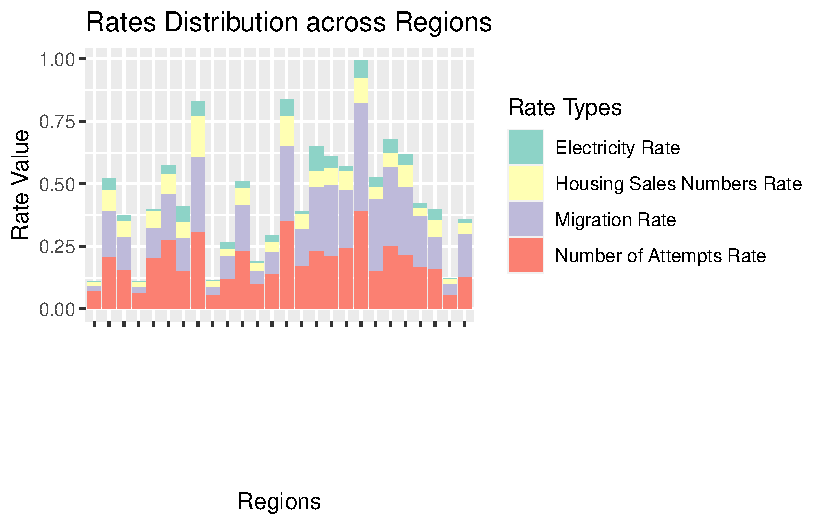
\includegraphics{analysis_files/figure-pdf/unnamed-chunk-12-2.pdf}

}

\end{figure}

The high education level of the Marmara Region may cause electricity
consumption to be high in this region. However, other regions appear to
have lower-than-expected electricity consumption. While high usage is
expected due to illegal electricity use, especially in Eastern Anatolia,
the data do not support this prediction.

Since the Aegean Region is a summer resort, it was expected that house
sales would be high. The fact that Southeastern Anatolia has the lowest
housing sales rates is an expected result due to the development level
of the region.

Number of Initiatives and Touristic Regions: The fact that the Black Sea
is a region with an unexpectedly high number of initiatives may be due
to the fact that it is a touristic region. This supports our prediction,
as the Aegean Region ranks second as a touristic region. It is
relatively expected that Southeastern Anatolia has the lowest number of
startups. The fact that the Black Sea is a region with an unexpectedly
high number of initiatives may be due to the fact that it is a touristic
region. This supports our prediction, as the Aegean Region ranks second
as a touristic region. It is relatively expected that Southeastern
Anatolia has the lowest number of startups.

When looking at correlation analyses, although the correlation between
electricity consumption and migration rates has the highest value, this
relationship cannot be said to be linear. The observed high value of the
correlation between education level and electricity consumption (close
to 1) supports that high education level may be related to electricity
consumption. We obtained results that support our opinion stated in
first sentence.

In the analyzes made on a regional basis, no significant relationship is
seen. It is observed that each region is associated with different data
sets at different levels compared to the other.

\hypertarget{workforce-and-usable-income}{%
\subsection{Workforce and Usable
Income}\label{workforce-and-usable-income}}

\begin{Shaded}
\begin{Highlighting}[]
\FunctionTok{ggplot}\NormalTok{(region26, }\FunctionTok{aes}\NormalTok{(}\AttributeTok{x =}\NormalTok{ workforce15plus, }\AttributeTok{y =}\NormalTok{ usableincome, }\AttributeTok{label =}\NormalTok{ region2id)) }\SpecialCharTok{+}
\FunctionTok{geom\_point}\NormalTok{(}\AttributeTok{color =} \StringTok{"blue"}\NormalTok{, }\AttributeTok{size =} \DecValTok{3}\NormalTok{) }\SpecialCharTok{+} 
\FunctionTok{geom\_text}\NormalTok{(}\AttributeTok{vjust =} \SpecialCharTok{{-}}\FloatTok{0.5}\NormalTok{, }\AttributeTok{hjust =} \SpecialCharTok{{-}}\FloatTok{0.5}\NormalTok{) }\SpecialCharTok{+}
\FunctionTok{labs}\NormalTok{(}\AttributeTok{title =} \StringTok{"Workforce ve Usable Income"}\NormalTok{, }\AttributeTok{x =} \StringTok{"Workforce"}\NormalTok{, }\AttributeTok{y =} \StringTok{"Usable Income"}\NormalTok{)}
\end{Highlighting}
\end{Shaded}

\begin{figure}[H]

{\centering 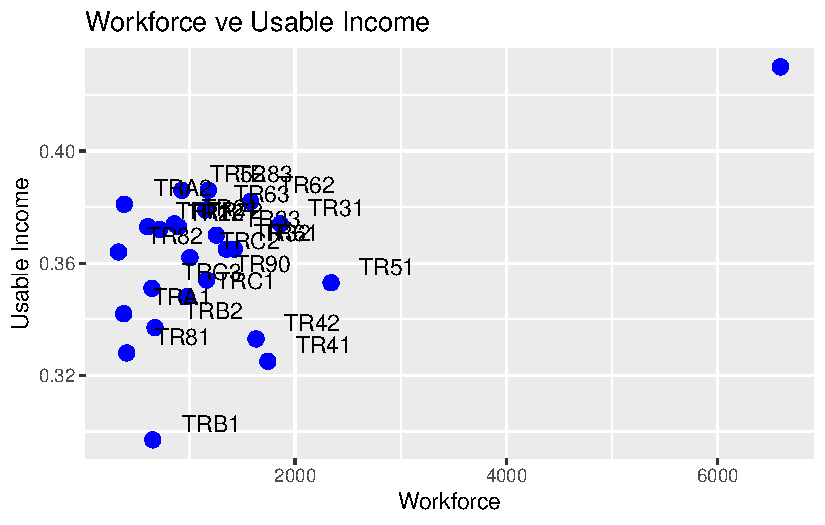
\includegraphics{analysis_files/figure-pdf/unnamed-chunk-13-1.pdf}

}

\end{figure}



\end{document}
